%% Преамбула TeX-файла

% 1. Стиль и язык
\documentclass[utf8x, 14pt]{G7-32} % Стиль (по умолчанию будет 14pt)

% Остальные стандартные настройки убраны в preamble-std.tex
\sloppy

% 1. Настройки стиля ГОСТ 7-32
% Для начала определяем, хотим мы или нет, чтобы рисунки и таблицы нумеровались в пределах раздела, или нам нужна сквозная нумерация.
% А не забыл ли автор букву 't' ?
\EqInChapter % формулы будут нумероваться в пределах раздела
\TableInChapter % таблицы будут нумероваться в пределах раздела
\PicInChapter % рисунки будут нумероваться в пределах раздела

% 2. Добавляем гипертекстовое оглавление в PDF
\usepackage[
bookmarks=true, colorlinks=true, unicode=true,
urlcolor=black,linkcolor=black, anchorcolor=black,
citecolor=black, menucolor=black, filecolor=black,
]{hyperref}

% 3. Изменение начертания шрифта --- после чего выглядит таймсоподобно.
% apt-get install scalable-cyrfonts-tex

\IfFileExists{cyrtimes.sty}
    {
        \usepackage{cyrtimespatched}
    }
    {
        % А если Times нету, то будет CM...
    }


% 4. Прочие полезные пакеты.
\usepackage{underscore} % Ура! Теперь можно писать подчёркивание.
                        % И нельзя использовать подчёркивание в файлах.
                        % Выбирай, но осторожно.

\usepackage{graphicx}   % Пакет для включения рисунков

\usepackage{tikz}

 % 5. Любимые команды
\newcommand{\Code}[1]{\textbf{#1}}

% 6. Поля
% С такими оно полями оно работает по-умолчанию:
% \RequirePackage[left=20mm,right=10mm,top=20mm,bottom=20mm,headsep=0pt]{geometry}
% Если вас тошнит от поля в 10мм --- увеличивайте до 20-ти, ну и про переплёт не забывайте:
\geometry{right=20mm}
\geometry{left=30mm}


% 7. Tikz
\usepackage{tikz}
\usetikzlibrary{arrows,positioning,shadows}

% 8 Листинги

\usepackage{listings}

% Значения по умолчанию
\lstset{
  basicstyle= \footnotesize,
  breakatwhitespace=true,% разрыв строк только на whitespacce
  breaklines=true,       % переносить длинные строки
%   captionpos=b,          % подписи снизу -- вроде не надо
  inputencoding=koi8-r,
  numbers=left,          % нумерация слева
  numberstyle=\footnotesize,
  showspaces=false,      % показывать пробелы подчеркиваниями -- идиотизм 70-х годов
  showstringspaces=false,
  showtabs=false,        % и табы тоже
  stepnumber=1,
  tabsize=4,              % кому нужны табы по 8 символов?
  frame=single
}

% Стиль для псевдокода: строчки обычно короткие, поэтому размер шрифта побольше
\lstdefinestyle{pseudocode}{
  basicstyle=\small,
  keywordstyle=\color{black}\bfseries\underbar,
  language=Pseudocode,
  numberstyle=\footnotesize,
  commentstyle=\footnotesize\it
}

% Стиль для обычного кода: маленький шрифт
\lstdefinestyle{realcode}{
  basicstyle=\scriptsize,
  numberstyle=\footnotesize
}

% Стиль для коротких кусков обычного кода: средний шрифт
\lstdefinestyle{simplecode}{
  basicstyle=\footnotesize,
  numberstyle=\footnotesize
}

% Стиль для BNF
\lstdefinestyle{grammar}{
  basicstyle=\footnotesize,
  numberstyle=\footnotesize,
  stringstyle=\bfseries\ttfamily,
  language=BNF
}

% Определим свой язык для написания псевдокодов на основе Python
\lstdefinelanguage[]{Pseudocode}[]{Python}{
  morekeywords={each,empty,wait,do},% ключевые слова добавлять сюда
  morecomment=[s]{\{}{\}},% комменты {а-ля Pascal} смотрятся нагляднее
  literate=% а сюда добавлять операторы, которые хотите отображать как мат. символы
    {->}{\ensuremath{$\rightarrow$}~}2%
    {<-}{\ensuremath{$\leftarrow$}~}2%
    {:=}{\ensuremath{$\leftarrow$}~}2%
    {<--}{\ensuremath{$\Longleftarrow$}~}2%
}[keywords,comments]

% Свой язык для задания грамматик в BNF
\lstdefinelanguage[]{BNF}[]{}{
  morekeywords={},
  morecomment=[s]{@}{@},
  morestring=[b]",%
  literate=%
    {->}{\ensuremath{$\rightarrow$}~}2%
    {*}{\ensuremath{$^*$}~}2%
    {+}{\ensuremath{$^+$}~}2%
    {|}{\ensuremath{$|$}~}2%
}[keywords,comments,strings]

% Подписи к листингам на русском языке.
\renewcommand*\thelstnumber{\oldstylenums{\the\value{lstnumber}}}
\renewcommand\lstlistingname{\cyr\CYRL\cyri\cyrs\cyrt\cyri\cyrn\cyrg}
\renewcommand\lstlistlistingname{\cyr\CYRL\cyri\cyrs\cyrt\cyri\cyrn\cyrg\cyri}

% Произвольная нумерация списков.
\usepackage{enumerate}

\usepackage{pdfpages}
\usepackage{longtable, multirow, rotating, color, colortbl}
\usepackage{amsmath}
\usepackage{tikz}
\usepackage{pgfplots}
\begin{document}

\frontmatter % выключает нумерацию ВСЕГО; здесь начинаются ненумерованные главы: реферат, введение, глоссарий, сокращения и прочее

% Команды \breakingbeforechapters и \nonbreakingbeforechapters
% управляют разрывом страницы перед главами.
% По-умолчанию страница разрывается.

% \nobreakingbeforechapters
% \breakingbeforechapters

\includepdf[pages=-]{inc/doc/titul.pdf}
\includepdf[pages=-]{inc/doc/task.pdf}
\includepdf[pages=-]{inc/doc/plan.pdf}



\tableofcontents


\Introduction

Зародившаяся в начале прошлого века с целью упорядочить работу телефонных станций, теория массового обслуживания нашла применения в моделировании самых разнообразных систем, таких как системы связи, обработки информации, снабжения, производства и др.

Несмотря на имеющиеся достижения в области математического исследования характеристик систем массового обслуживания, наиболее универсальным подходом по прежнему остается имитационное моделирование.

Язык имитационного моделирования GPSS создан специально для моделирования систем массового обслуживания и на данный момен является доминирующим в этой области. Однако, существующие версии систем имитационного моделирования на основе языка GPSS либо слишком дороги, либо ограничены в возможностях и не позволяют провести все необходимые исследования.\cite{KST} Помимо этого, на данный момент затруднено интегрирование моделей, разработанных при помощи GPSS в другие программные средства (напимер, в целях оптимизации параметров исследуемой системы).

Целью данной работы является создание системы имитационного моделирования, основанной на принципах и синтаксисе GPSS, однако позволяющей разрабатывать модели как часть более крупной программы.

В качестве языка разработки был выбран Haskell. Haskell является динамично развивающимся функциональным языком проограммирования, который получает все больше сторонников во всем мире, в том числе и в России. \cite{HaskellRef}. Для Haskell характерны строгая статическая типизация, модульность, строгое разделение функций на чистые и не чистые, ленивые вычисления, функции высших порядков и др.\cite{Haskell} Помимо этого использование языка Haskell позволит производить описание систем при помощи синтаксиса схожего с синтаксисом GPSS, при этом разработанные модели будут являться объектами первого класса, что позволит, например, передать модель как параметр в функцию оптимизации.

Для достижения поставленной цели необходимо решить следующие задачи:
\begin{itemize}
\item изучить принципы функционирования и синтаксис описания моделей в GPSS;
\item разработать синтаксис описания моделей схожий с синтаксисом GPSS, но при этом позволяющий составлять модели в виде функций языка Haskell;
\item выбрать подмножество блоков GPSS, которые следует реализовать в системе;
\item реализовать алгоритмы описания моделей и имитационного моделирования;
\item разработать и реализовать транслятор моделей GPSS в формат разработанной системы моделиования;
\item провести тестирование разработанного программного обеспечения;
\item провести моделирование некоторой эталонной системы массового обслуживания в разработанной системе, GPSS и аналитически и убедиться в совпадении полученных результатов.
\end{itemize}



\mainmatter % это включает нумерацию глав и секций в документе ниже


\chapter{Аналитический раздел}
\label{cha:analysis}

В данном разделе проводится обзор принципов функционирования и синтаксиса системы GPSS, а также производится выбор подмножества возможностей GPSS, которые следует реализовать в разрабатываемой системе.

\section{Краткий обзор GPSS}

GPSS стал одним из первых языков моделирования, облегчающих процесс написания имитационных программ. Он был создан в виде конечного продукта Джефри Гордоном в фирме IBM в 1962~г.\cite{ImitGPSS} В свое время он входил в десятку лучших языков программирования и по сей день широко используется для решения практических задач. Наиболее современной версией GPSS для персональных компьютеров на данный момент является пакет GPSS World, разработанный компанией Minuteman Software.

Описание системы на GPSS представляет собой последовательность блоков,
каждый из которых соответствует некоторому оператору (подпрограмме). Каждый блок
имеет определенное количество параметров (полей).


Основой имитационных алгоритмов GPSS является дискретно-событийный подход~--- моделирование системы в дискретные моменты времени, когда происходят события, отражающие последовательность изменения состояний системы во времени.\cite{ImitGPSS}

\section{Объекты языка GPSS}

Основными Объектами языка GPSS являются транзакты и блоки, которые отображают соответственно динамические и статические объекты моделируемой системы.

Транзакты~--- динамические элементы GPSS-модели. В реальной системе транзактам могут соответствовать такие элементы как заявка, покупатель автомобиль и др. Состояние транзакта в процессе моделирования характеризуется следующими атрибутами:

\begin{enumerate}
\item параметры~--- набор значений связанных с транзактом. Каждый транзакт может иметь произвольное число параметров. Каждый параметр имеет уникальный номер, по которому на него можно сослаться;
\item приоритет~--- определяет порядок продвижения транзактов при конкурировании за общий ресурс;
\item текущий блок~--- номер блока, в котором транзакт находится в данный момент;
\item следующий блок~--- номер блока, в который транзакт попытается войти;
\item время появления транзакта~---  момент времени в который транзакт был создан;
\item состояние~--- состояние, показывающее в каких списках транзакт находится в данный момент. Транзакт может находиться в одном из следующих состояний:
    \begin{enumerate}
    \item активен~--- транзакт находится в списке текущих событий и имеет наивысший приоритет;
    \item приостановлен~--- транзакт находится в списке будущих событий либо в списке текущих событий, но с меньшим приоритетом;
    \item пассивен~--- транзакт находится в списке прерываний, списке синхронизации, списке блокировок или списке пользователя;
    \item завершен~--- транзакт уничтожен и больше не участвует в модели.
    \end{enumerate}
    Диаграмма состояний транзакта показана на Рисунке~\ref{fig:transactionState}.
\end{enumerate}


\begin{figure}[ht]
  \centering
  \includegraphics[width=\textwidth]{inc/dia/transactionState}
  \caption{Состояния транзакта}
  \label{fig:transactionState}
\end{figure}


Блоки~--- статические элементы GPSS-модели. Модель в GPSS может быть представлена как диаграмма блоков, т.е. ориентированный граф, узлами которого являются блоки, а дугам~--- направления движения транзактов. с каждым блоком связано некоторое действие, изменяющее состояние прочих элементов модели. Транзакты проходят блоки один за другим, до тех пор пока не достигнут блока TERMINATE. В ряде случаев транзакт может быть остановлен в одном из блоков до наступления некоторого события.


Помимо транзактов и блоков в GPSS используются следующие объекты: устройства, многоканальные устройства (хранилища, памяти), ключи, очереди, списки пользователя и др.


\section{Управления процессом моделирования в GPSS}

В системе GPSS интерпретатор поддерживает сложные структуры организации списков (см. Рисунок~\ref{fig:GPSSChains}).\cite{ImitGPSS} Два основных из них~--- список текущих событий (СТС) и список будущих событий (СБС).

\begin{figure}[ht]
  \centering
  \includegraphics[width=\textwidth]{inc/dia/gpss}
  \caption{Списки GPSS}
  \label{fig:GPSSChains}
\end{figure}

В СТС входят все события запланированные  на текущий  момент модельного времени. Интерпретатор в первую очередь просматривает этот список и перемещает по модели те транзакты, для которых выполнены все условия. Если таких транзактов в списке не оказалось интерпретатор обращается к СБС. Он переносит все события, запланированные на ближайший момент времени и вновь возвращается к просмотру СТС. Перенос также осуществляется в случае совпадения текущего момента времени с моментом наступления ближайшего события из СБС.

В целях эффективной организации просмотра транзактов, движение которых заблокировано (например, из-за занятости некоторого ресурса), используются следующие вспомогательные списки:

\begin{itemize}
\item списки блокировок~--- списки транзактов, которые ожидают освобождения некоторого ресурса;
\item список прерываний~--- содержит транзакты, прерванные во время обслуживания. Используется для организации обслуживания одноканальных устройств с абсолютным приоритетом;
\item списки синхронизации~--- содержат транзакты одного семейства (созданные блоком SPLIT), которые ожидают синхронизации в блоках (MATCH, ASSEMBLE или GATHER);
\item списки пользователя~--- содержат транзакты, выведенные пользователем из СТС с помощью блока LINK. Транзакты могут быть возвращены в СТС помощью блока UNLINK.
\end{itemize}




\section{Выбор подмножества реализуемых блоков}

В современной версии языка GPSS (входящей в пакет GPSS World) поддерживается 53 различных блока.\cite{GPSSRef} В рамках данной работы не представляется возможным реализовать  аналоги каждого из них. Поэтому следует выделить некоторое подмножество блоков, которое с одной не будет слишком обширным, а с другой~--- позволит решать практические или по крайней мере учебные задачи.

В качестве примера рассмотрим задачу из курса Модели оценки качества аппаратно программных комплексов:

\begin{quote}
В вычислительной системе, содержащей N процессоров и M каналов обмена данными, постоянно находятся K задач. Разработать модель, оценивающую производительность системы с учетом отказов и восстановлений процессоров и каналов. Имеется не более L ремонтных бригад, которые ремонтируют отказывающие устройства с бесприоритетной  дисциплиной. Интенсивность отказов, восстановлений, средние времена обработки сообщения и среднее время обдумывания также известны.
\end{quote}

Схема модели данной системы показана на Рисунке~\ref{fig:mainModel}

\begin{figure}[ht]
\centering
\includegraphics[width=\textwidth]{inc/dia/main}
\caption{Схема моделируемой системы}
\label{fig:mainModel}
\end{figure}

Как и подавляющее большинство других задач, данная задача, безусловно, не может быть решена без использования блоков GENERATE, TERMINATE и ADVANCE. Так как моделируемая система является замкнутой, при описании модели не обойтись без блока TRANSFER.

К сожалению, не представляется возможным реализовать процессоры и каналы как многоканальные устройства, т.к. многоканальные устройства в GPSS не поддерживают абсолютные приоритеты и не позволяют смоделировать выход из строя отдельных каналов устройства. Однако, требуемую систему можно описать при помощи множества одноканальных устройств и блока TRANSFER в режиме ALL. Таким образом, также понадобятся блоки SEIZE и RELEASE. Для моделирования отказов устройств можно воспользоваться блоками FAVAIL и FUNAVAIL либо блоками PREEMPT и RETURN.

Наконец, доступные ремонтные бригады можно смоделировать с помощью многоканального устройства. Соответственно, понадобятся блоки ENTER и LEAVE.

Приблизительная модель системы показана в Листинге~\ref{lst:sample01}

\lstinputlisting[caption=Приблизительная модель системы,label=lst:sample01]{inc/src/analysModel.gpss}

Таким образом, разрабатываемая система имитационного моделирования должна поддерживать аналоги по крайней мере следующих блоков: ADVANCE, ENTER, GENERATE, LEAVE, PREEMPT, RELEASE, RETURN, SEIZE, TERMINATE и TRANSFER.

\section{Описание выбранных блоков}

Ниже представлено описание выбранных блоков в соответствии со справочным руководством GPSS World.\cite{GPSSRef}

\subsection*{ADVANCE A,B}

Блок ADVANCE осуществляет задержку продвижения транзактов на заданный промежуток времени.

A~--- Среднее время задержки. Не обязательный параметр. Значение по умолчанию~---~0.

B~--- Максимально допустимое отклонение времени задержки либо функция-модификатор.

\subsection*{ENTER A,B}

При входе в блок ENTER транзакт либо занимает заданное количество каналов указанного многоканального устройства либо блокируется до его освобождения.

A~--- Имя или номер многоканального устройства. Обязательный параметр.

B~--- Число требуемых каналов. Не обязательный параметр. Значение по умолчанию~--- 1.

\subsection*{GENERATE A,B,C,D,E}

Блок GENERATE предназначен для создания новых транзактов.

A~--- Среднее время между генерацией последовательных заявок. Не обязательный параметр.

B~--- Максимальное допустимое отклонение времени генерации либо функция-модификатор. Не обязательный параметр.

С~--- Задержка до начала генерации первого транзакта. Не обязательный параметр.

D~--- Ограничение на максимальное допустимое число созданных транзактов. Не обязательный параметр. Пол умолчанию ограничение отсутствует.

E~--- Уровень приоритета создаваемых заявок. Не обязательный параметр. Значение по умолчанию~--- 0.

\subsection*{LEAVE A,B}

При входе в блок LEAVE транзакт освобождает заданное число каналов указанного многоканального устройства.

A~--- Имя или номер многоканального устройства. Обязательный параметр.

B~--- Число требуемых каналов. Не обязательный параметр. Значение по умолчанию~--- 1.

\subsection*{PREEMPT A,B,C,D,E}

Блок PREEMPT подобен блоку SEIZE и вошедший в него транзакт также пытается занять указанное одноканальное устройство. Однако, данный блок позволяет транзакту занять устройство, даже если в данный момент оно уже занято другим транзактом, при соблюдении ряда условий, определяемых параметрами блока.

A~--- Имя или номер одноканального устройства. Обязательный параметр.

B~--- задает режим работы блока. PR~--- режим приоритетов. По умолчанию~--- режим прерываний. В режиме прерываний транзакт может вытеснить из устройства любой другой транзакт, если тот в свою очередь не захватил устройство через блок PREEMPT. В режиме приоритетов транзакт может вытеснить любой транзакт с меньшим приоритетом.

C~--- задает номер блока, куда будет направлен транзакт вытесненный и устройства в результате действия блока PREEMPT. 

D~--- задает номер параметра вытесненного транзакта, в  котором будет сохранено время, которое осталось транзакту до окончания обработки а устройстве.

E~--- задает режим удаления вытесненного транзакта. RE~--- вытесненное сообщение удаляется из устройства и более не претендует на владение им. Требует обязательного указания параметра C. Значение по умолчанию~--- вытесненный транзакт будет вновь пытаться занять устройство. 

\subsection*{RELEASE A}

Блок RELEASE освобождает одноканальное устройство.

A~--- Имя или номер одноканального устройства. Обязательный параметр.

\subsection*{RETURN A}

Блок RELEASE освобождает одноканальное устройство.

A~--- Имя или номер одноканального устройства. Обязательный параметр.

\subsection*{SEIZE A}

При входе в блок SEIZE транзакт занимает указанное одноканальное устройство либо блокируется до его освобождения.

A~--- Имя или номер одноканального устройства. Обязательный параметр.

\subsection*{TERMINATE A}

Блок TERMINATE завершает поступивший в него транзакт. И опционально уменьшает счетчик завершенных транзактов. Когда счетчик достигает нуля имитация останавливается.

A~--- Значение, на которое следует уменьшить счетчик завершенных транзактов. Не обязательный параметр. Значение по умолчанию~--- 0.

\subsection*{TRANSFER A,B,C,D}

Блок TRANSFER является основным средством позволяющим изменить маршрут транзакта и перенаправить его к произвольному блоку модели. Параметр A определяет режим работы блока. Смысл остальных параметров меняется в зависимости от выбранного режима.

\paragraph{Безусловный режим}. Если параметр А пропущен, то блок TRANSFER работает в безусловном режиме. Входящий в блок TRANSFER транзакт переходит к блоку, указанному в поле В.

\paragraph{Статистический режим}. Параметр А является числом от 0 до 1, показывающим какая доля транзактов перейдет к блоку, указанному в параметре С. Остальные транзакты переходят к блоку,ь указанному в параметре B.

\paragraph{Режим BOTH}. Если параметр А равен BOTH, то блок TRANSFER работает в одноименном режиме.В этом режиме каждый входящий транзакт сначала пытается перейти к блоку, указанному в поле В. Если это сделать не удается, транзакт пытается перейти к блоку, указанному в поле С. Если транзакт не сможет перейти ни к тому, ни к другому блоку, он остается в блоке TRANSFER и будет повторять в том порядке попытки перехода при каждом просмотре списка текущих событий, до тех пор, пока не сможет выйти из блока TRANSFER.

\paragraph{Режим ALL}. Если параметр А равен ALL, то блок TRANSFER работает в одноименном режиме.В этом режиме каждый входящий транзакт1 прежде всего пытается перейти к блоку, указанному в поле В. Если транзакт не может войти в этот блок, то последовательно проверяются все блоки в определенном ряду в поисках первого, способного принять это сообщение, включая последний блок, указанный операндом С. Номер каждого проверяемого блока вычисляется как сумма номера предыдущего блока и шага, заданного операндом D. По умолчанию значение операнда D принимается равным 1.

\paragraph{Режим PICK}. Если параметр А равен PICK, то блок TRANSFER работает в одноименном режиме. Этот режим подобен режиму ALL, за тем исключением, что блок назначения выбирается случайным образом с одинаковой вероятностью.

\section{Выводы}

Был проведен обзор устройства системы GPSS и осуществлен выбор подмножества блоков, необходимых для моделирования не сложных систем массового обслуживания. Представлено описание назначения и параметров каждого из выбранных блоков.



\chapter{Конструкторский раздел}

В данном разделе проводится выбор синтаксиса описания моделей в разрабатываемой системе, описываются алгоритмы и структуры данных, используемые при формировании моделей и непосредственно при моделировании, а также проводится построение аналитической и имитационной модели учебной системы описанной в предыдущем разделе.



\section{Требования к синтаксису}

Синтаксис разрабатываемой системы должен быть, на сколько это возможно, схож с синтаксисом системы GPSS. 

Программа на языке GPSS представляет из себя последовательность операторов, каждый из которых описывает тот или иной элемент модели (функцию, блок, устройство и др.). Этот подход естественен для императивных языков программирования, в которых программа является последовательностью команд, меняющих состояние программы. Однако Haskell относится к категории функциональных языков, программы на которых описываются как функции, значение которых вычисляется. При этом нет фиксированной, заданной программистом, последовательности операций, которые должны быть выполнены для достижения результата. 

Тем не менее, в языке Haskell предусмотрен механизм, позволяющий описать конкретную последовательность вычислений~--- монады. В сочетании с так называемой do-нотацией, этот механизм позволит проводить описание моделей на Haskell, используя синтаксис схожий с GPSS.

\section{Монады}

Понятие монады в языке Haskell основано на теории категорий. В рамках данной теории монада может быть определена (не вполне строго) как моноид в категории эндофункторов. Однако для практического использования этого понятия в рамках языка Haskell можно обойтись менее формальным определением.

В соответствии с \cite{Haskell} монада~--- это контейнерный тип данных (то есть такой, который содержит в себе значения других типов), представляющий собой экземпляр класса Monad определенного в модуле Prelude. 

Под классом в Haskell, понимается не тип данных, как в объектно-ориентированных языках, а набор методов (функций), которые применимы для работы с теми или иными типами данных, для которых объявлены экземпляры заданных классов. Наиболее близким аналогом классам в Haskell являются интерфейсы в таких языках как Java или C\#. Более точно их следует называть классами типов, но т.к. в данной работе используется исключительно функциональная парадигма, в дальнейшем для краткости они будут называться просто классами.

Значения монад можно воспринимать, как значения м некоторым дополнительным контекстом. В случае монады Maybe значения обладают дополнительным контекстом того, что вычисления могли закончиться неуспешно. Монада IO добавляет контекст, указывающий что получение значений связано с действиями ввода/вывода и потому не является детерминированным и может иметь побочные эффекты. В случае списков (которые также являются монадой) контекстом является то, что значение может являться множественным или отсутствовать.

Класс Monad определен в модуле Prelude следующим образом:

\lstinputlisting[caption=Класс Monad,label=lst:monad]{inc/src/Monad.hs}

Функция \Code{return}\footnote{Следует отметить, что название return никак нельзя назвать удачным, так как оно неизбежно вызывает ассоциации с одноименным оператором из многих императивных языков программирования, на которые она не похожа ничем кроме названия. Данная функция не завершает выполнение функции, а лишь оборачивает переданное значение в монаду.} преобразует переданное ей значение типа a  в монадическое значение типа m a. Другими словами она помещает значение в некоторый контекст по умолчанию, в зависимости от выбранной монады. Для списка это будет список из одного элемента, для монады IO~--- действие ввода вывода, всегда возвращающее заданное значение и не имеющее побочных эффектов и т.д.

Функция \Code{$>>=$} определяет операцию связывания. Она принимает монадическое значение и передает его функции, которая принимает обычное значение и возвращает монадическое. При этом сохраняется накопленный контекст и к нему добавляется новый, полученный в результате выполнения функции.

Функция \Code{$>>$} также предназначена для связывания и используется в тех случаях, когда переданное монадическое значение не представляет интереса, а значение имеет только переданный с ним контекст вычислений. Для этой функции в классе определена реализация по умолчанию, по этому в большинстве случаев при определении экземпляра класса Monad в явном виде ее не реализуют.

Функция \Code{fail} никогда не вызывается программистом явным образом и предназначена для обработки неуспешного окончания вычислений при сопоставлении с образцом в do-нотации, что позволяет избежать аварийного завершения программы и вернуть неудачу в контексте текущей монады.

\section{Нотация do}

Так как монады находят крайне широкое применение в программах на языке Haskell (в первую очередь, без использования монады IO невозможно осуществить ввод/вывод), в синтаксис языка было добавлено специальное ключевое слово \Code{do}, призванное упростить написание монадических функций, сделать их более читаемыми и избавить от излишнего <<синтаксического мусора>>.

Если в коде программы встречается конструкция с ключевым словом \Code{do}, то транслятор выполняет следующие преобразования\footnote{В приведенных преобразованиях используются управляющие символы \Code{;}, \Code{\{} и \Code{\}}, хотя в реальных программах на языке Haskell их можно встретить довольно редко. Это связано с тем, что в Haskell используется так называемый <<двумерный синтаксис>>: при правильной расстановке отступов, транслятор самостоятельно расставляет точки с запятой и фигурные скобки и в большинстве случаев нет смысла загромождать ими исходный код. Тем не менее в случае необходимости их можно расставить и явным образом.}:

\begin{verbatim}
1. do {e} → e
2. do {e; es} → e >> do {es}
3. do {let decls; es} → let decls in do {es}
4. do {p <- e; es} → let ok p = do {es}
                          ok _ = fail "..."
                      in e >>= ok
\end{verbatim}

При помощи нотации \Code{do} приведенный ниже фрагмент кода

\begin{verbatim}
foo :: Maybe String
foo = Just 3 >>= (\x -> Just "!" >>= (\y -> Just (show x ++ y)))}
\end{verbatim}

может быть записан в следующей более читаемой форме:

\begin{verbatim}
foo :: Maybe String
foo = do x <- Just 3 
         y <- Just "!" 
         return (show x ++ y)
\end{verbatim}

\section{Монада State}

Часто в процессе вычислений возникает необходимость хранить и изменять некоторое состояние, в зависимости от которого результат вычислений может меняться. Haskell является чистым функциональным языком программирования функции должны быть детерминированы и не иметь побочных эффектов, поэтому текущее состояние обычно передается в функции как еще один параметр, а возвращает функция пару из собственно результата и обновленного состояния.

Для того, чтобы упростить написание функций оперирующих некоторым состоянием в Haskell была введена монада \Code{State}. Она определена в модуле \Code{Control.Monad.State} следующим образом:

\begin{verbatim}

newtype State s a = State {runState :: s -> (a, s)}

instance Monad (State s) where
    return x = State $ \s -> (x,s)
    (State h) >>= f = State $ \s -> let (a, newState) = h s
                                        (State g) = f a
                                    in g newState

\end{verbatim}

Функция \Code{return} создает вычисление с состоянием, которое всегда возвращает один и тот же результат и оставляет переданное в него состояние без изменений. Функция \Code{$>>=$} <<склеивает>> два вычисления с состоянием так, что конечное  состояние первого становится начальным для второго, а результат и конечное состояние второго вычисления становятся также результатом и конечным состоянием итогового, составного вычисления.

Помимо этого для работы с монадой \Code{State} используются две вспомогательные функции \Code{put} и \Code{get}. Функция \Code{put} является вычислением, которое устанавливает состояние в заданное значение не зависимо от его предыдущего значения и не возвращает никакого результата (точнее возвращает кортеж нулевой длины \Code{()}). Функция \Code{get} возвращает текущее состояние и оставляет его без изменений. 

\section{Описание модели как вычисление с состоянием}

Описание модели на языке GPSS представляет из себя последовательность блоков. В Haskell такое описание удобно представить как последовательность функций, каждая из которых добавляет к уже сформированной модели очередной блок. 

Такой процесс удобно представить как вычисление с состоянием. Каждая функция, формирующая блок, помимо параметров самого блока должна принимать текущее состояние~--- список уже сформированных к данному моменту боков в порядке их формирования. В качестве результата функция возвращает новое состояние~--- модель к которой добавлен только что сформированный блок (см. Рисунок \ref{fig:StateIDEF}).

\begin{figure}[ht]
  \centering
  \includegraphics[width=\textwidth]{inc/dia/StateIDEF}
  \caption{Процесс формирования модели}
  \label{fig:StateIDEF}
\end{figure}

Для реализации такого механизма целесообразно воспользоваться монадой \Code{State}, что позволит скрыть явную передачу состояния от одной функции к другой. А использование нотации \Code{do} сделает описание модели почти идентичным синтаксису GPSS:

\begin{verbatim}

model = 
    do generate (10,2)
       advance 3
       terminate 1

\end{verbatim}


\section{Функции формирования блоков}

В языке GPSS имена всех блоков пишутся с заглавной буквы. Параметры отделяются от имени блока пробелом и разделяются запятыми. Синтаксис Haskell не позволяет в точности повторить эти соглашения. Имена функций в Haskell обязаны начинаться со строчной буквы. Параметры функций обычно разделяются пробелами и не берутся в скобки (каррированные функции) либо заключаются в скобки и разделяются запятыми (не каррированные функции)\footnote{Строго говоря все функции в Haskell принимают ровно один параметр. Функции от N параметров на самом деле принимают один параметр и возвращают функцию от N-1 параметра (каррированные функции) либо принимают параметр-кортеж (некаррированные).}. Оба варианта описания параметров одинаково близки к синтаксису GPSS и можно выбрать любой из них, однако для второго варианта существенно легче реализовать перегрузку функций.

\section{Состояние транзакта}

Основным объектом в процессе моделирования является транзакт. Моделирование представляет собой передвижение транзактов от блока к блоку, в процессе которого могут изменяться состояния тех или иных объектов системы (обслуживающих аппаратов, очередей, хранилищ).

Параметры, определяющие состояние транзакта приведены в таблице~\ref{tab:transactionState}

\begin{table}
\caption{Параметры состояния транзакта}
\label{tab:transactionState}
\begin{tabular}{|l|l|p{0.6\textwidth}|}
\hline
Имя параметра & Тип &Описание \\
\hline
currentBlock & Int & Номер блока модели, в котором в данный момент находится транзакт.\\
\hline
nextBlock & Int & Номер блока в который транзакт попытается перейти.\\
\hline
priority & Int & Приоритет транзакта.\\
\hline
params & IntMap Double & Массив параметров транзакта.\\
\hline
ownership & String & Имя устройства, на котором в данный момент обрабатывается транзакт.\\
\hline
\end{tabular}
\end{table}

Также как часть состояния транзакта моет рассматриваться информация о том, в каком из глобальных или локальных списков событий он находится в данный момент. Так как в каждый момент транзакт должен находиться только в одном из списков, хранить ту информацию в отдельном поле не целесообразно.

\section{Состояния объектов системы}

В процессе перемещения по блокам транзакты изменяют состояния других объектов системы. Эти состояния во-первых, в свою очередь, оказывает влияние на движение транзактов, а во-вторых предназначено для сбора статических данных в процессе моделирования.

Параметры состояний обслуживающих аппаратов, хранилищ и очередей приведены в таблицах~\ref{tab:facState},~\ref{tab:storState} и \ref{tab:queueState} соответственно.

\begin{table}
\caption{Параметры состояния обслуживающего аппарата}
\label{tab:facState}
\begin{tabular}{|l|l|p{0.6\textwidth}|}
\hline
Имя параметра & Тип & Описание \\
\hline
idAvailable & Bool & Флаг, показывающий доступно или занято в данный момент обслуживающее устройство\\
\hline
toInterupted & Bool & Флаг, показывающий, захватил ли, обрабатывающийся в данный момент транзакт, устройство обычным образом или путем вытеснения обрабатывавшегося до этого транзакта.\\
\hline
captureCount & Int & Счетчик, показывающий сколько раз было захвачено данной устройство.\\
\hline
captureTime & Double & Суммарное время, в течение которого устройство было занято.\\
\hline
lastCaptureTime & Double & Момент времени, когда устройство было захвачено в последний раз.\\
\hline
utilization & Double & Процент времени, в течении которого устройство было занято.\\
\hline
ownerPriority & Int & Приоритет транзакта, обслуживающегося на устройстве в данный момент. \\
\hline
dc & [Transaction] & Список заявок, ожидающих освобождения устройства. \\
\hline
ic & \parbox{25mm}{[(Maybe Double,\\Transaction)] }  & Список заявок, вытесненных с устройства и ожидающих его освобождения для продолжения обслуживания.\\
\hline
pc & [Transaction] & Список заявок, не сумевших вытеснить, обрабатываемый в данный момент транзакт, и ожидающих освобождения устройства.\\
\hline
\end{tabular}
\end{table}


\begin{table}
\caption{Параметры состояния хранилища}
\label{tab:storState}
\begin{tabular}{|l|l|p{0.65\textwidth}|}
\hline
Имя параметра & Тип & Описание \\
\hline
capacity & Int & Емкость хранилища.\\
\hline
unused & Int & Число доступных единиц ресурса в хранилище.\\
\hline
avgInUse & Double & Среднее число занятых единиц ресурса.\\
\hline
useCount & Int & Число захватов ресурса за время моделирования.\\
\hline
lastMod & Double & Момент последнего захвата или освобождения ресурса.\\
\hline
utilization & Double &Средний процент захваченных единиц ресурса.\\
\hline
maxInUse & Int & Максимальное число одновременно захваченных единиц ресурса. \\
\hline
dc & [Transaction] & Список заявок, ожидающих освобождения достаточного числа ресурсов хранилища. \\
\hline
\end{tabular}
\end{table}


\begin{table}
\caption{Параметры состояния очереди}
\label{tab:queueState}
\begin{tabular}{|l|l|p{0.65\textwidth}|}
\hline
Имя параметра & Тип & Описание \\
\hline
currentContent & Int & Число заявок в очереди в данный момент модельного времени.\\
\hline
maximumContent & Int & Максимальное число заявок в очереди за все время моделирования.\\
\hline
averageContent & Double & Среднее число заявок в очереди.\\
\hline
lastChangeTime & Double & Момент времени, когда в последний раз заявка встала в очередь или покинула ее.\\
\hline
\end{tabular}
\end{table}


\section{Состояние системы в целом}

В процессе имитационного моделирования система последовательно переходит из одного состояния в другое, до тех пор, пока не будет достигнуто некоторое условие остановки моделирования. В данном случае моделирование происходит до тех пор, пока в блоках TERMINATE не будет завершено заданное число транзактов.

Состояние моделируемой системы может быть описано параметрами, указанными в таблице~\ref{tab:simState}. Моделирование продолжается до тех пор, пока значение параметра \Code{toTerminate} не достигнет нуля.

Отношения перечисленных сущностей показаны на рисунке~\ref{fig:umlSim}.

\begin{figure}[ht]
  \centering
  \includegraphics[width=\textwidth]{inc/dia/er}
  \caption{Отношения между сущностями системы}
  \label{fig:umlSim}
\end{figure}


\begin{table}[ht!]
\caption{Параметры состояния системы}
\label{tab:simState}
\begin{tabular}{|l|l|p{0.5\textwidth}|}
\hline
Имя параметра & Тип & Описание \\
\hline
currentTime & Double & Текущий момент модельного времени.\\
\hline
toTerminate & Int & Число транзактов, которое необходимо завершить для окончания моделирования.\\
\hline
blocks & Array Int SBlock & Список блоков, составляющих модель.\\
\hline
facilities & Map String Facility & Список состояний обслуживающих аппаратов.\\
\hline
storages & Map String Storage & Список состояний хранилищ.\\
\hline
queues & Map String Queue & Список состояний очередей.\\
\hline
cec & [Transaction] & Список будущих событий~--- список транзактов, продвижение которых требует наступления некоторого момента модельного времени. Упорядочен по возрастанию ожидаемого момента времени. \\
\hline
fec & [(Double,Transaction)] & Список текущих событий~--- список транзактов, продвижение которых возможно в данный момент модельного времени. Упорядочен по убыванию приоритета транзактов. \\
\hline
\end{tabular}
\end{table}


\section{Алгоритм имитационного моделирования}

Процесс моделирования запускается при вызове функции, одним параметром которой является сформированная модель, а вторым~--- количество транзактов, которое необходимо завершить для окончания моделирования.  Схема алгоритма показана на рисунке~\ref{fig:simFlowchart}.

\begin{figure}[ht!]
  \centering
  \includegraphics[height=0.7\textheight]{inc/dia/simFlowchart}
  \caption{Алгоритм имитационного моделирования}
  \label{fig:simFlowchart}
\end{figure}

На первом шаге алгоритма происходит активация всех блоков GENERATE. Для каждого из них вычисляется время создания ближайшего транзакта и эти транзакты помещаются в список будущих событий.

На втором шаге из списка будущих событий извлекаются события, наступающие в ближайший момент модельного времени. Модельное время передвигается на момент наступления тих событий, а сами события помещаются в  список текущих событий. 

На третьем шаге, до тех пор пока список текущих событий не опустеет, происходит продвижение транзакта из того списка с наибольшим приоритетом. Продвижение каждого транзакта происходит до тех пор, пока транзакт тем или иным образом не покинет текущий список (например, войдет в блок ADVANCE и будет помещен в список будущих событий или попытается войти в блок занятого устройства и попадет в список транзактов, ожидающих освобождения того устройства).

Шаги два и три повторяются до тех пор, пока в процессе моделирования не будет завершено заданное число транзактов.




\section{Обработка захода транзакта в блок}

Каждый раз, когда заявка пытается зайти в очередной блок, вызывается функция обработчик, которая определяет, может ли транзакт это сделать и какие дополнительные действия при этом должны быть выполнены. Исключением является блок GENERATE, для которого обработчик (определяющий время создания нового транзакта) вызывается при выходе из него транзакта. 

Обработчики индивидуальны для каждого типа блоков. В качестве примера на рисунках~\ref{fig:enterFlowchart} и \ref{fig:leaveFlowchart} показаны алгоритмы обработчиков блоков ENTER и LEAVE соответственно.

\begin{figure}[ht!]
  \centering
  \includegraphics[width=\textwidth]{inc/dia/enterFlowchart}
  \caption{Алгоритм обработки блока ENTER}
  \label{fig:enterFlowchart}
\end{figure}

\begin{figure}[ht!]
  \centering
  \includegraphics[width=\textwidth]{inc/dia/leaveFlowchart}
  \caption{Алгоритм обработки блока LEAVE}
  \label{fig:leaveFlowchart}
\end{figure}

При входе транзакта в блок ENTER проверяется количество свободных единиц ресурса в соответствующем хранилище. Если ресурса достаточно, то транзакт успешно входит в блок, количество доступных ресурсов уменьшается и обновляется статистика использования хранилища. Затем транзакт продолжает движение по блокам. Если же транзакту требуется больше ресурсов, чем в данный момент есть в хранилище, транзакт попадает в список транзактов, ожидающих освобождения ресурсов.

При входе транзакта в блок LEAVE освобождается указанное количество ресурсов соответствующего хранилища и транзакт продолжает движение по блокам. Если есть транзакты, ожидающие освобождения ресурса, среди них выбирается транзакт с наибольшим приоритетом и делается попытка выделить ему необходимое количество ресурса. Если это удается, то транзакт помещается в список текущих событий, в противном случае он возвращается в список ожидания.

\section{Структура библиотеки}

На рисунке~\ref{fig:libStruct} показана общая структура спроектированной библиотеки.

\begin{figure}[ht!]
  \centering
  \includegraphics[width=\textwidth]{inc/dia/libStructHuge}
  \caption{Структура разработанной библиотеки}
  \label{fig:libStruct}
\end{figure}

На диаграмме можно выделить:


\begin{itemize}
\item {Модуль содержащий непосредственно алгоритм имитационного моделирования.}
\item {Группу модулей с обработчиками захода транзактов в те или иные блоки.}
\item {Модуль формирующий результаты моделирования на основе заключительного состояния системы.}
\item {Группу модулей предназначенных для формирования моделируемой системы и содержащие функции добавляющие в систему те или иные блоки.}

\end{itemize}

\section{Демонстрационная программа}

Для демонстрации возможностей спроектированной библиотеки, а также с целью удостовериться  в адекватности выбранных алгоритмов моделирования и верности их реализации, целесообразно разработать демонстрационную программу. 

Проектируемая программа должна проводить решение приведенной в предыдущем разделе задачи аналитически и при помощи разработанной библиотеки при различных входных параметрах и выводить результаты в удобной для сравнения форме. Целесообразно также предусмотреть возможность автоматического варьирования выбранного параметра модели и построения графика зависимости результата от этого параметра при фиксированных прочих для аналитической и имитационной модели.

Предполагаемая структура такой программы показана на рисунке~\ref{fig:demoStruct}.

\begin{figure}[ht]
  \centering
  \includegraphics[width=\textwidth]{inc/dia/demoStruct}
  \caption{Структура демонстрационной программы}
  \label{fig:demoStruct}
\end{figure}

\section{Аналитическая модель системы}

Ниже представлен способ аналитического вычисления характеристик системы приведенной в предыдущем разделе.При выводе формул использовались методы укрупнения модели и укрупнения состояний описанные в~\cite{Kurov}.

\subsection{Моделирование отказов и восстановлений}
Состояние системы можно описать вектором $ \xi (t) = (\xi_{1}(t),\,\xi_{2}(t))$, где $\xi_{1}(t)$~--- число неисправных процессоров в момент времени $t$, $\xi_{2}(t)$~--- число неисправных каналов в момент времени $t$.

На рисунке~\ref{fig:broke-graph} показана структура фрагмента графа состояний системы, где $\beta_{ij}=\beta\frac{i}{i+j}min\left\lbrace i+j,L\right\rbrace$, $\delta_{ij}=\delta\frac{j}{i+j}min\left\lbrace i+j,L\right\rbrace$. 
\begin{figure}[ht]
\centering
\includegraphics[height=6cm]{inc/dia/broke-graph}
\caption{Структура фрагмента графа состояний системы}
\label{fig:broke-graph}
\end{figure}

Проведем укрупнение состояний системы. Объединим в одно макросостояние все вершины графа, у которых одинаковым является первый компонент $\xi_{1}(t)$~--- число неисправных процессоров. Полученный граф представлен на рисунке~\ref{fig:broke-proc}, где $\beta_i=\beta\sum\limits_{j=0}^N\pi_j\frac{i}{i+j}min\left\lbrace i+j,L\right\rbrace$, $\pi_j$~--- вероятность того, что отказали ровно j каналов.

\begin{figure}[ht]
\centering
\includegraphics[width=\textwidth]{inc/dia/broke-proc}
\caption{Граф состояний системы}
\label{fig:broke-proc}
\end{figure}

Тогда выражения для определения вероятностей стационарных состояний примут вид:

\begin{equation}
\label{eq:broke-proc}
\left\{
   \begin{array}{lcl}
	p_{0} = \left( 1 + \dfrac{M \alpha}{\beta_1} +  ... + \dfrac{M! \alpha^{M}}{\prod \limits_{i=1}^M \beta_i} \right) ^{-1} \\
	p_{i} = p_{0} \dfrac{\alpha^{i}\prod \limits_{j=1}^{i} (M-j+1)}{\prod \limits_{j=1}^i \beta_{j}}, \quad i = \overline{1,M}  \\ 
	\beta_i=\beta\sum\limits_{j=0}^N\pi_j\frac{i}{i+j}min\left\lbrace i+j,L\right\rbrace
   \end{array}
\right.
\end{equation}
 
Аналогичным образом объединим в одно макросостояние все вершины графа, у которых одинаковым является второй компонент $\xi_{2}(t)$~--- число неисправных каналов. Полученный граф представлен на рисунке~\ref{fig:broke-chan}, а выражения для определения вероятностей стационарных состояний примут вид:

\begin{equation}
\label{eq:broke-chan}
\left\{
   \begin{array}{lcl}
	\pi_{0} = \left( 1 + \dfrac{N \gamma}{\delta_1} +  ... + \dfrac{N! \gamma^{N}}{\prod \limits_{i=1}^N \delta_i} \right) ^{-1} \\
	\pi_{i} = \pi_{0} \dfrac{\gamma^{i}\prod \limits_{j=1}^{i} (N-j+1)}{\prod \limits_{j=1}^i \delta_{j}}, \quad i = \overline{1,N}  \\ 
	\delta_j=\delta\sum\limits_{i=0}^M p_i\frac{j}{i+j}min\left\lbrace i+j,L\right\rbrace
   \end{array}
\right.
\end{equation}

\hfill

\begin{figure}[ht]
\centering
\includegraphics[width=\textwidth]{inc/dia/broke-chan}
\caption{Граф состояний системы}
\label{fig:broke-chan}
\end{figure}

\hfill

Применяя формулы~\ref{eq:broke-proc} и~\ref{eq:broke-chan} итеративно получим вероятности отказов процессоров и каналов в системе. В качестве начального приближения можно взять $\pi_i=\frac{1}{M}$

\hfill

\subsection{Укрупнение модели}

\hfill

Заменим исходную модель агрегированной однофазной моделью АМ1 (см. рисунок~\ref{fig:AM1}). В агрегированный узел объединена подсистема, включающая в себя процессоры и каналы. Интенсивность обслуживания в этом узле зависит от числа находящихся в нем заявок.

\hfill

\begin{figure}[ht]
\centering
\includegraphics[height=7cm]{inc/dia/AM1}
\caption{Укрупненная модель АМ1}
\label{fig:AM1}
\end{figure}

\hfill

Граф состояний полученной системы представлен на рисунке~\ref{fig:graphAM1}. Производительность системы может быть вычислена по формулам:


\begin{equation}
\label{eq:AM1}
\left\{
   \begin{array}{lcl}
	\hat{\pi}_{0} = \left( 1 + \dfrac{K \lambda}{\xi_1} +  ... + \dfrac{K! \lambda^{K}}{\prod \limits_{i=1}^K \xi_i} \right) ^{-1} \\
	\hat{\pi}_{i} = \hat{\pi}_{0} \dfrac{\lambda^{i}\prod \limits_{j=1}^{i} (K-j+1)}{\prod \limits_{j=1}^i \xi_{j}}, \quad i = \overline{1,K}  \\ 
	\xi_{ср}^{*}=\sum \limits_{i=1}^K \xi_i \hat{\pi_i}
   \end{array}
\right.
\end{equation}


\begin{figure}[ht]
\centering
\includegraphics[width=\textwidth]{inc/dia/graphAM1}
\caption{Граф состояний модели АМ1}
\label{fig:graphAM1}
\end{figure}

Однако, чтобы воспользоваться приведенными формулами, необходимо знать параметры связи $\mu_i$. Чтобы их найти, рассмотрим укрупненную модель АМ2, структура и граф состояний которой показаны на рисунках~\ref{fig:AM2} и~\ref{fig:graphAM2}. За состояние системы примем количество заявок на процессорной фазе, а интенсивности переходов могут быть выражены по формулам:

\begin{equation}
\label{eq:mu}
\mu_i = \mu \sum \limits_{j=0}^M p_j min \left\lbrace i, M-j \right\rbrace
\end{equation}

\begin{equation}
\label{eq:nu}
\nu_i = \nu \sum \limits_{j=0}^N \pi_j min \left\lbrace n-i+1, N-j \right\rbrace
\end{equation}



\begin{figure}[ht]
\centering
\includegraphics[height=7cm]{inc/dia/AM2}
\caption{Укрупненная модель АМ2}
\label{fig:AM2}
\end{figure}

\begin{figure}[ht]
\centering
\includegraphics[width=\textwidth]{inc/dia/graphAM2}
\caption{Граф состояний модели АМ2}
\label{fig:graphAM2}
\end{figure}


Параметр связи может вычислен по следующим формулам:


\begin{equation}
\label{eq:AM2}
\left\{
   \begin{array}{lcl}
	\hat{p}_{0} = \left( 1 + \dfrac{\nu_1}{\mu_1} +  ... + \dfrac{\prod \limits_{i=1}^n \nu_i}{\prod \limits_{i=1}^n \mu_i} \right) ^{-1} \\
	\hat{p}_{i} = \hat{p}_{0} \dfrac{\prod \limits_{j=1}^{i} (\nu_j)}{\prod \limits_{j=1}^i \mu_{j}}, \quad i = \overline{1,n}  \\ 
	\xi_n = \sum \limits_{i=1}^n \hat{p}_i \mu_i
   \end{array}
\right.
\end{equation}


\subsection{Окончательная расчетная схема}
Последовательность расчета производительности системы должна быть следующей (см. рисунок~\ref{fig:idefAnalit}):

\begin{enumerate}
\item По формулам~\ref{eq:broke-proc} и ~\ref{eq:broke-chan} вычислить $\pi_i, i=\overline{0,N}$ и $p_i, i=\overline{0,M} $.
\item По формулам~\ref{eq:mu},~\ref{eq:nu} и~\ref{eq:AM2} вычислить $\xi_n, n=\overline{1,K}$.
\item Вычислить $\xi^{*}$ по формулам~\ref{eq:AM1}.
\end{enumerate}


\begin{figure}[ht!]
\centering
\includegraphics[width=0.9\textheight,angle=-90]{inc/dia/idefAnalit}
\caption{Последовательность расчета производительности системы}
\label{fig:idefAnalit}
\end{figure}

\section{Имитационная модель}

Ниже представлена имитационная модель демонстрационной системы, реализованная при помощи разработанной системы моделирования.

\subsection{Моделирование многоканальных обслуживающих устройств}

Так как в исследуемой системе используются многоканальные обслуживающие устройства, каждый из каналов которых может выйти из строя независимо от других, не представляется возможным промоделировать их при помощи хранилищ (хранилища могут быть отключены только целиком и не поддерживают вытеснение транзактов). Поэтому придется каждый канал обслуживающего устройства моделировать отдельным многоканальным устройством, а выбор транзактом свободного канала осуществлять при помощи блока TRANSFER, работающего в режиме ALL.

Ниже приведен код функции, формирующий часть модели, ответственную за обслуживание заявки на одном из процессоров. В качестве параметров функция принимает номер процессора, интенсивность обработки и метку блока с которого начинается следующая фаза обслуживания.

\begin{verbatim}
proc i mu l =
    do seize ("proc" ++ show i)
       advance (1/mu, xpdis)
       release ("proc" ++ show i)
       transfer ((),l)
\end{verbatim}

\subsection{Моделирование отказов и восстановлений}

Для моделирования отказов и восстановления каждого из каналов используется отдельный транзакт, который сперва захватывает соответствующее устройство при помощи блока PREEMPT в режиме прерывания (после этого устройство становится недоступно для транзактов, моделирующих задачи), после этого пытается захватить ресурс хранилища, моделирующего ремонтные бригады, и после того через некоторое время освобождает устройство и ресурс (устройство восстановлено и снова доступно для обработки задач). Время, остававшееся до окончания обработки транзакту, вытесненному в момент поломки, сохраняется в  параметре транзакта, а сам транзакт перенаправляется на фазу дообслуживания.


Ниже приведен код функции, формирующей часть модели ответственную за отказы и восстановления одного из процессоров. В качестве параметров функция принимает номер процессора, интенсивности его отказов и восстановлений и метку блока, с которого начинается фаза дообслуживания.

\begin{verbatim}
breakReairProc i alpha beta l' = 
    do generate (0,0,0,1)
       l <- advance (1/alpha, xpdis)
       preempt ("proc" ++ show i, (), l', 1, RE)
       enter "repairers"
       advance (1/beta,xpdis)
       return' ("proc" ++ show i)
       leave "repairers"
       transfer ((),l)
\end{verbatim}

Функция формирующая фазу дообслуживания во всем подобна функции \Code{proc} за исключением того, что время обслуживания берется из параметра транзакта, а не определяется случайным образом.

\begin{verbatim}
procFinish i l =
    do seize ("proc" ++ show i)
       advance (Pr 1)
       release ("proc" ++ show i)
       transfer ((),l)
\end{verbatim}

\subsection {Общая модель системы}

Функция формирующая при помощи вышеописанных общую модель системы показана ниже. В качестве параметров она принимает все параметры системы (количество задач, процессоров, каналов и ремонтных бригад и интенсивности обработки на различных фазах и отказов и восстановлений).

\begin{verbatim}
model m n k l lambda mu nu alpha beta gamma delta = 
    do storage ("repairers", l)
       generate (0,0,0,1)
       advance 100
       terminate 1
       
       generate (0,0,0,k)
       userPhase <- advance (1/lambda, xpdis)
       seize "counter"
       release "counter"
       procStart <- transfer (All,userPhase +5, 
                              userPhase + 5 + (m-1)*4,4)
       chanStart <- transfer (All,userPhase +5+4*m, 
                              userPhase + 5 + m*4 + (n-1)*4,4)
       mapM_ (\i -> proc i mu chanStart) [1..m]
       ls <- mapM (\i -> chan i nu userPhase) [1..n]
       
       let l = fromIntegral $ last ls
       procFinishL <- transfer (All,l + 3,
                                l + 3 + (m-1)*4,4)
       chanFinishL <- transfer (All,l + 3 + 4*m,
                                l + 3 + 4*m + (n-1)*4,4)
       mapM_ (\i -> procFinish i chanStart) [1..m]
       mapM_ (\i -> chanFinish i userPhase) [1..n]
       
       when (alpha > 0) $ mapM_ (\i -> breakReairProc 
                                         i alpha beta procFinishL
                                ) [1..m]
       when (gamma > 0) $ mapM_ (\i -> breakReairChan 
                                         i gamma delta chanFinishL
                                ) [1..n]
\end{verbatim}

 Первым делом функции объявляется хранилище емкостью равной числу ремонтных бригад. Затем создается группа блоков ответственная за ограничение времени моделирования.

Последующие блоки отвечают за создание транзактов, моделирующих задачи пользователей и время их обдумывания пользователем. Далее следуют блоки TRANSFER предназначенные для передачи заявки на свободный в данный момент процессор или канал. Далее путем многократного вызова функций \Code{proc} и \Code{chan} формируется часть модели ответственная за обработку задач на процессорной и канальной фазах. 

Далее аналогичным образом, при помощи блоков TRANSFER и многократного вызова функций \Code{procFinish} и \Code{chanFinish} формируются фазы дообслуживания. 

И в заключение при помощи функций \Code{breakReairProc} и \Code{breakReairChan} формируются блоки моделирующие отказы и восстановления.

\section{Выводы}

В результате проектирования был разработан синтаксис и алгоритм описания моделей, а также алгоритмы и структуры данных необходимые для имитационного моделирования. Были спроектированы структуры библиотеки имитационного моделирования и демонстрационной программы, призванной проиллюстрировать ее работу. Были разработаны аналитическая и имитационная модели демонстрационной системы, описанной в предыдущем разделе.


\chapter{Технологический раздел}

В данном разделе описывается реализация разработанной системы и демонстрационной программы, средстава разработки, сборки и развертывания, а также тестирование.

\section{Выбор средств программной реализации}

Так как целью работы является разработка библиотеки для языка Haskell, целесообразно вести разработку на этом же языке. Язык Haskell относится к функциональным языкам общего назначения и обладает следующими особенностями:

\begin{itemize}
\item Чистые функции. Большинство функций в языке Haskell являются чистыми, то есть детерминированными и не имеющими побочных эффектов. При использовании таких функций программист может быть уверен, что при вызове такой функции не будет произведено каких-либо неявных действий (запись даных в файл, изменение значения переданных параметров, изменеие состояния некоторого объекта и т.п.) и на одних и тех же входны параметрах функкция всегда вернет одинаковый результат. Это существенно упрощает разраотку и тестирование программ.

\item Ленивые вычисления. Все вычисления в Haskell по умолчанию являются ленивыми, то есть ни одно значение не будет вычислено до тех пор, пока его значение действительно не понадобится. Этот механизм позволяет экономить выислительные мощности и работать со структурами вроде бесконечных списков. Однако при неаккураьном использовании это может привести к неэффективному расходованию памяти.

\item Строгая статическая типизация. Строгая типизация позволяет писать более надежные программы, так как несоответствие типов приведет к сообщению об ошибке, а не к некорректному поведению программы и будет быстрее обнаружено и исправлено. Статическая типизация позволяет выявить такие ошибки еще на этапе компиляции программы.

\item Автоматическое управление памятью. Как и большинство современных языков программирования Haskell берет на себя выделение и освобождение памяти. Это гарантировать отсутствие в разрабатываемой программе таких ошибок как переполнение буфера, неинициализированные переменные и т.п.

\end{itemize}

Помимо этого для Haskell существует обширный централизованный архив библиотек Hackage\cite{hackage}, и поисковая система Hoogl\cite{hoogle}, позволяющая найти описание функции не ттолько по ее названи но и по сигнатуре.

\subsection{Построение графиков}

Для построения графиков была выбрана система Gnuplot\cite{gnuplot}. Это свободно распространяемая, кросплатформенная программа предназначенная для построения двух- и трехмерных графиков функций, заданных как аналитически, так и в виде наборов данных. Gnuplot поддержвает вывод результатов в различных форматах: растровых (PNG, JPEG), векторных (SVG, PDF), в виде кода LaTeX, в интерактивном режиме и др. Система используется для построения графиков в таких математических пакетах как GNU Octave, Maxima и других.

Для использования возможностей Gnuplot в программах на Haskell существует несколько библиотек, опубликованных на Hackage. В данной работе была использована библиотека EasyPlot.


\subsection{Построение пользовательского интерфейса}

Для построения пользовательского интерфейса демонстрационной программы была использована библиотека wxHaskell\cite{wxhaskell}, которая в свою очередь является оберткой вокруг библиотеки для построения пользовательского интерфейса на C++ wxWidgets. 

Особенности wxWidgets:

\begin{itemize}
\item Созданные с помощью данной библиотеки приложения переносимы на большинство современных ОС.

\item В разработанном интерфейсе используются элементы управления привычные для пользователей целевой ОС. То есть стиль интерфейса программы будет отличаться на различных ОС и будет соответствовать рекомендуемому стилю для конкретной системы.

\end{itemize}

wxHaskell является надстройкой над wxWidgets, позволяющей создавать графический интерфейс к программам на языке Haskell. Она поддерживает большую часть функционала wxWidgets, позволяет описывать интерфейс в <<декларативном>> стиле с использованием функциональных связок и абстракцй высокого уровня. Библиотека особенно удобна для создания демонстрационных версий программ, так как во многом берет на себя решение адачи корректного расположения элементов управления на экране. 

\subsection{Сборка и развертывание библиотеки}

Для сборки разработанной библиотеки и развертывания ее на целевой машине была использована система Cabal. Данная система предоставляет единый интерфейс для создания и установки инсталяционных пакетов с программами и библиотеками на Haskell. Система связана с архивом библиотек Hackage и позволяет устанавливать хранящиеся там пакеты и оформить собственную программу в виде пакета для Hackage.

Информация о создаваемом пакете указывается в файле \Code{.cabal} в директории проекта. В нем указываются:
    
\begin{itemize}
\item имя пакета;

\item текущая версия;

\item информация об авторе и лицензии;

\item допустимые версии компилятора;

\item используемые расширения компилятора;

\item входящие в состав пакета библиотеки и исполняемые программы;

\item пакеты Hackage, необходимые для работы пакета;

\item и др.

\end{itemize}
    
    
Фрагмент файла \Code{.cabal} для разработаной библиотеки приведен ниже.

\lstinputlisting[caption=Фрагмент описания пакета,label=lst:cabal]{inc/src/.cabal}

Сборка и установка пакета выполняется следующими командами:

\begin{itemize}
\item \Code{cabal configure}~--- подготовка к сборке программы: определение целевой платформы, зависимостей и др.;

\item \Code{cabal build}~--- запуск процесса компиляции;

\item \Code{cabal install}~--- установка пакета в систему. Включает в себя первые две комманды;

\item \Code{cabal clean}~--- удаляет все временные файлы созданные предыдущими коммандами;

\end{itemize}
    
    

%\section{Демонстрационная программа}

%Для демонстрации возможностей разработанной библиотеки, а также в целях дополнительного тестирования была разработанна демонстрационная программа. В программе производится расчет производительности системы массового обслуживания при заданных параметрах и варьировании одного из них. Расчет производительности ведется как путем имитационного моделирования при помощи разработанной бибилиотеки, так и с помощью аналитической модели. Программа выводит на экран графики, позвооляющие сравнить значения полученные путем моделирования с полученными теоретически. Структура разработанной программы показа на рисунке~\ref{fig:demoStruct}



\section{Тестирование}

Для модульного тестирования разработанной библиотеки использовалась библиотека HUnit\cite{HUnit}. Это фреймворк основанный на идеях JUnit, но предназначенный для тестированя программ на Haskell.

Типичный базовый тест состоит из текстового описания, вычисляемого выражения и ожидаемого результата. Базовые тесты объединяются в группы, те, в свою очередь, могут объединяться в большие группы и т.д. В итоге образуется единая древовидная структура тестов. Ниже показан пример описания теста.

\begin{verbatim}
emptyFEC = TestCase (assertEqual "for (addFE [] (1,defTransact))," 
                                 ([(1,defTransact)]) 
                                 (addFE [] (1,defTransact))
                    )
\end{verbatim}

По результатам выполнения тестов HUnit выводит следующую статистику: общее число тестов, число проведенных тестов, число тестов вызвавших непредвиденное исключение (что говорит об ошибке в самом тесте) и число тестов, закончившихся неудачей (что обычно говорит об ошибке в тестируемой программе).

В таблице~\ref{tab:chainsTest} приведен протокол тестирования функции \Code{addFE}, добавляющей новое событие в список будущих событий.


\begin{table}[h!]
\caption{}
\label{tab:chainsTest}
\begin{tabular}{|l|p{0.7\textwidth}|}
\hline
Название теста & emptyFEC\\
\hline
Описание теста & Добавление события в пустой список\\
\hline
Ожидаемый результат & Список из одного события\\
\hline
Результат & Тест пройден\\
\hline
\hline
Название теста & nearestAddFE\\
\hline
Описание теста & Добавление в список события с наименьшим временем наступления\\
\hline
Ожидаемый результат & Добавленное событие становится первым в списке\\
\hline
Результат & Тест пройден\\
\hline
\hline
Название теста & lastAddFE\\
\hline
Описание теста & Добвление в списко события с наибольшим временем наступления\\
\hline
Ожидаемый результат & Добавленное событие становится последним в списке\\
\hline
Результат & Тест пройден\\
\hline
\hline
Название теста & middleAddFE\\
\hline
Описание теста & Добавление в список события с промежуточным временем наступления\\
\hline
Ожидаемый результат & Добавленное событие занимает место в списке в соответствии со своим временем наступления\\
\hline
Результат & Тест пройден\\
\hline
\hline
Название теста & multyAddFE\\
\hline
Описание теста & Добавление в список события с тем же  временем наступления, что и у  одного из событий в списке\\
\hline
Ожидаемый результат & Добавленное событие занимает место в списке сразу за событием с тем же временем наступления\\
\hline
Результат & Тест пройден \\
\hline
\end{tabular}
\end{table}

В общей сложности было проведено 84 теста. Вывод тестовой программы представлен ниже.

\begin{verbatim}
Cases: 84  Tried: 84  Errors: 0  Failures: 0
\end{verbatim}


\subsection{Тестирование стохастических функций}

При организации имитационного моделирования важную роль играют функции генерации случайных величин с заданным законом распределения. При тестировании таких функций приходится отказаться от описанного выше принципа <<выражение --- ожидаемое значение>>, поскольку результат вычисления функции различается от запуска к запуску.

Для тестирования таких функций следует многократно вычислить значение тестируемой функции и сравнить собранную статистику с ожидаемым распределением. В даннной работе в качестве критерия соответствия полученных значений ожидаемому распределению использовался критерий согласия Пирсона.

Для вычисления статистики по этому критерию и вычисления квантилей распределения $\chi^2$ и спользовался пакет statistics из архива библиотек Hackage.

\subsection{Сравнение аналитической и имитационной модели}

В качестве дополнительной проверки на корректность разработанных алгоритмов и безошибочность их реалиации был проведен ряд опытов с демонстрационной программой. Были построены графики зависимости производительности моделируемой системы от различных параметров при прочих фиксированных параметрах.

\subsection*{Опыт 1}

Варьируется число задач в системе. Количество процессоров и каналов равно единицы. Интенсивность обдумывания равна единице. Отказов и восстановлений нет. Интенсивности обработки на канальной и процессорной фазе равны 5. Результаты показаны на рисунке~\ref{fig:plot1}.

\begin{figure}[ht]
  \centering
  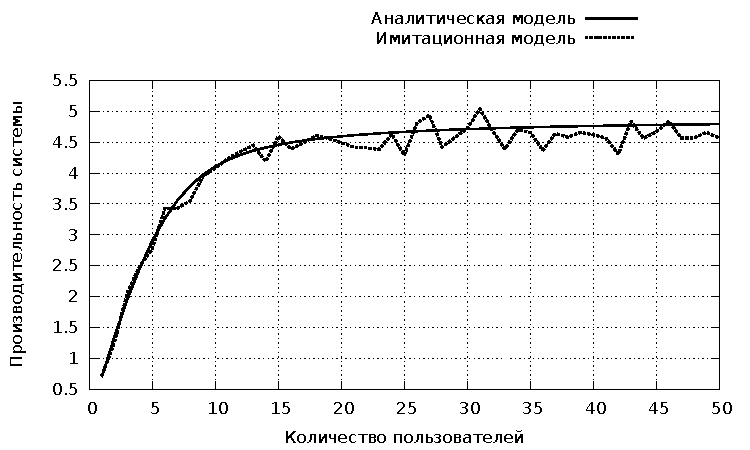
\includegraphics[width=\textwidth]{inc/pdf/plot1}
  \caption{Опыт 1}
  \label{fig:plot1}
\end{figure}

\subsection*{Опыт2}

Опыт проводится при тех же параметрах, но число каналов и интенсивность обслуживания на процессороной фаззе увеличены в двое. Результаты показаны на~\ref{fig:plot1a}.

\begin{figure}[ht]
  \centering
  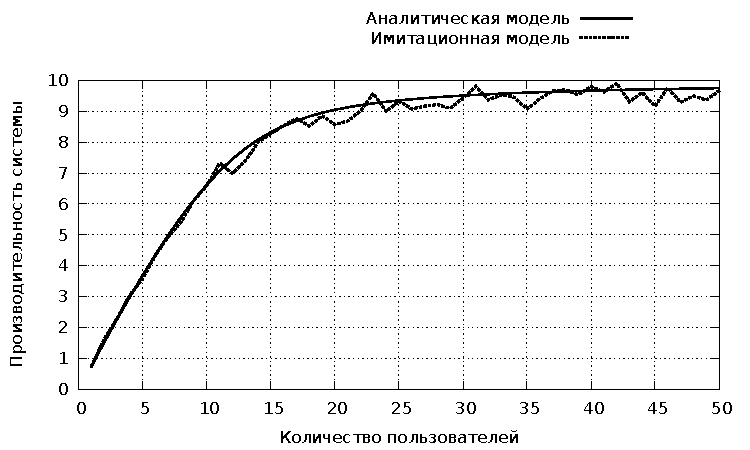
\includegraphics[width=\textwidth]{inc/pdf/plot1a}
  \caption{Опыт 2}
  \label{fig:plot1a}
\end{figure}


\subsection*{Опыт3}

Варьируется число процессоров. Число задач и каналов равняется 10. Итенсивность обдумывания равна единице. Интенсивности обработки задач на процессороной и канальной фазах равны 5. Результаты опыта показаны на рисунке~\ref{fig:plot2}.

\begin{figure}[ht!]
  \centering
  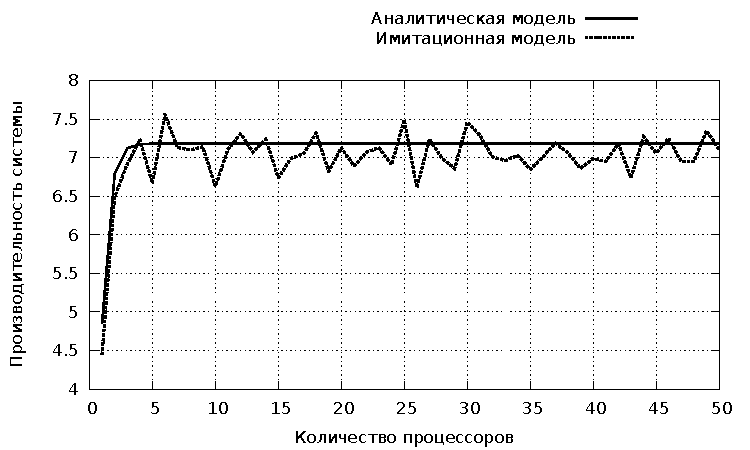
\includegraphics[width=\textwidth]{inc/pdf/plot2}
  \caption{Опыт 3}
  \label{fig:plot2}
\end{figure}

\subsection*{Опыт4}

Опыт проводится при тех же параметрах, что и предыдущий, но количество каналов уменьшено вдвое. Результаты опыта показаны на рисунке~\ref{fig:plot2a}.

\begin{figure}[ht!]
  \centering
  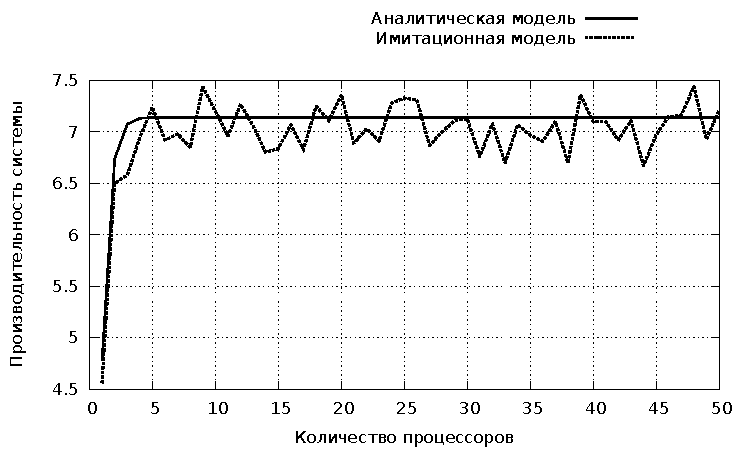
\includegraphics[width=\textwidth]{inc/pdf/plot2a}
  \caption{Опыт 4}
  \label{fig:plot2a}
\end{figure}

\subsection*{Опыт5}

Варьируется интенсивность обработки на канальной фазе. количество задач равно 10. Количество процессоров и каналов равно 4. Интенсивность обдумывания~--- 5, интенсивность обработки на процессорной фазе~--- 20 Результаты опыта показаны на рисунке~\ref{fig:plot3}.

\begin{figure}[ht!]
  \centering
  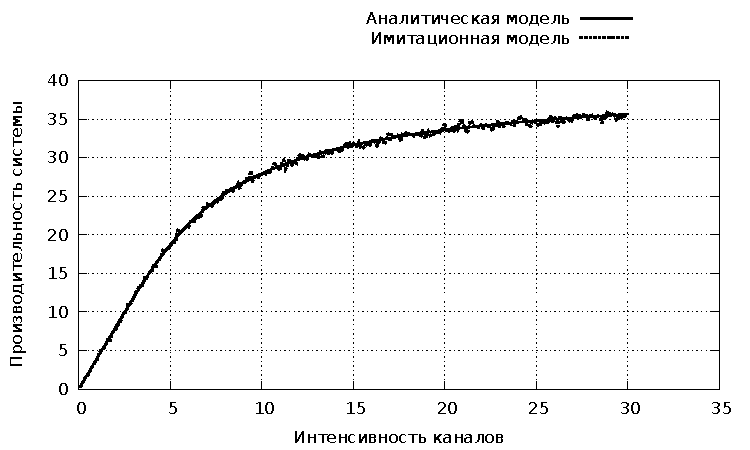
\includegraphics[width=\textwidth]{inc/pdf/plot3}
  \caption{Опыт 5}
  \label{fig:plot3}
\end{figure}

\subsection*{Опыт6}

Опыт проводится при тех же параметрах, что и предыдущий, но количество задач уменьшено вдвое. Результаты опыта показаны на рисунке~\ref{fig:plot3a}.

\begin{figure}[ht!]
  \centering
  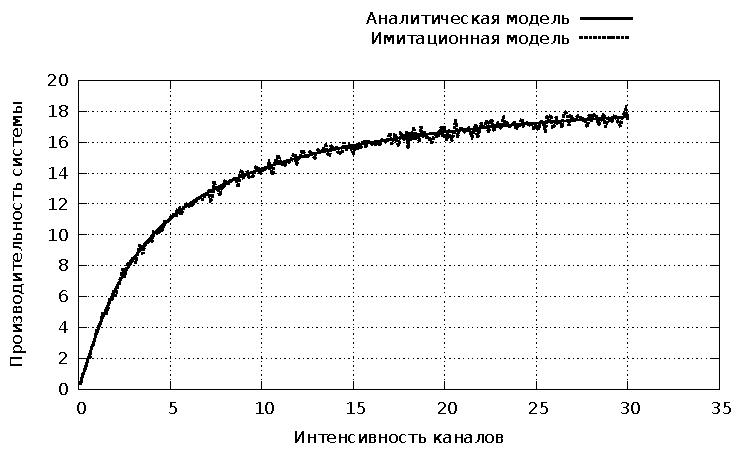
\includegraphics[width=\textwidth]{inc/pdf/plot3a}
  \caption{Опыт 6}
  \label{fig:plot3a}
\end{figure}

\subsection*{Опыт7}

Варьируется интенсивность отказов процессоров. Количество задач равно 10. Количество процессоров и каналов равно 4. Интенсивность обдумывания~--- 1, интенсивность обработки на процессорной  и канальной фазах~--- 3. Интенсивность восстановления процессоров равна 10. Количество ремонтных бригад~--- 5.Результаты опыта показаны на рисунке~\ref{fig:plot4}.


\begin{figure}[ht!]
  \centering
  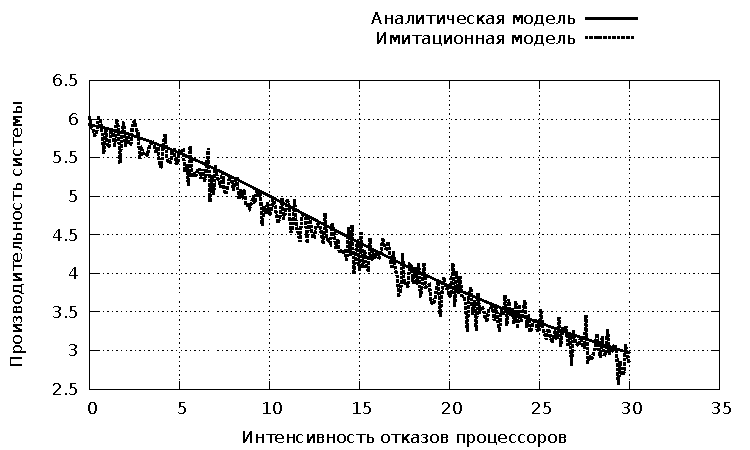
\includegraphics[width=\textwidth]{inc/pdf/plot4}
  \caption{Опыт 7}
  \label{fig:plot4}
\end{figure}

\subsection*{Опыт8}

Опыт проводится при тех же параметрах, что и предыдущий, но интенсивность восстановления процесоров уменьшена вдвое. Результаты опыта показаны на рисунке~\ref{fig:plot4a}.

\begin{figure}[ht!]
  \centering
  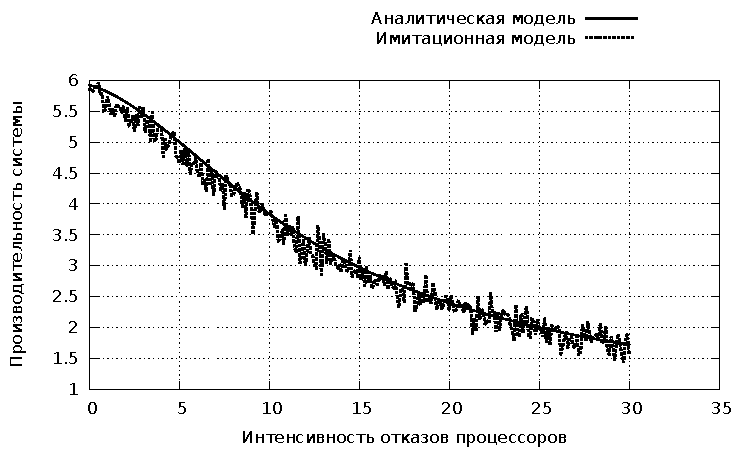
\includegraphics[width=\textwidth]{inc/pdf/plot4a}
  \caption{Опыт 8}
  \label{fig:plot4a}
\end{figure}

\subsection*{Опыт9}

Варьируется количество ремонтных бригад. Количество задач и процессоров~--- 5. Количество кканалов 15. Интенсивность обдумывания~---1. Интенсивность обработки на процессорной и канальной фазах~---5. Интенсивность отказов каналов~---14, интенсивность восстановлений~---7. Результаты опыта показаны на рисунке~\ref{fig:plot5}.

\begin{figure}[ht!]
  \centering
  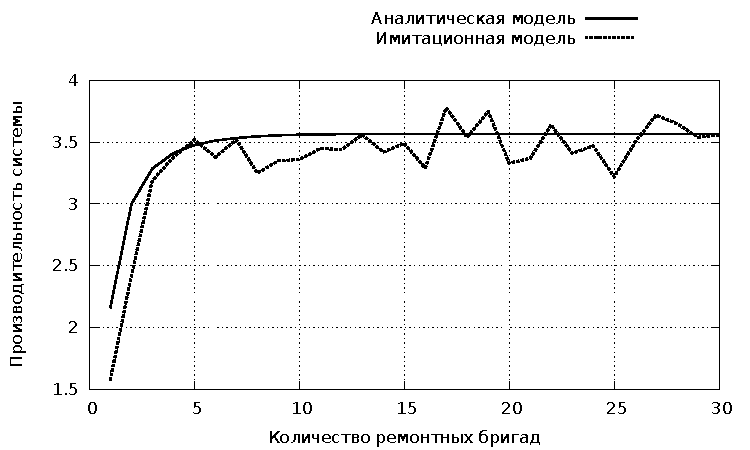
\includegraphics[width=\textwidth]{inc/pdf/plot5}
  \caption{Опыт 9}
  \label{fig:plot5}
\end{figure}

\subsection*{Опыт10}

Опыт проводится при тех же параметрах, что и предыдущий, но интенсивность восстановления взята равной интенсивности отказов. Результаты опыта показаны на рисунке~\ref{fig:plot5a}.

\begin{figure}[ht!]
  \centering
  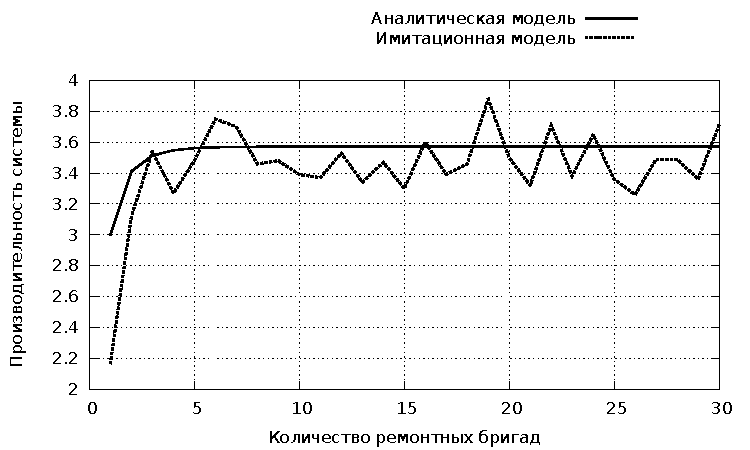
\includegraphics[width=\textwidth]{inc/pdf/plot5a}
  \caption{Опыт 10}
  \label{fig:plot5a}
\end{figure}

Из проведенных опытов видно, что данные полученные при помощи разработанной библиотеки и имитационной модели качественно соответствуют результатам анаолитических исследований. Некоторый разброс значений объясняется стохастическим характером модели.

\section{Выводы}

Были реализованы разработанные в предыдущем разделе методы и алгоритмы. Разработанная бибилиотека была протестирована при помощи модульного тестирования. Также был проведен ряд опытов подтверждащих адекватность построенной имитационной модели и корректность реализованных алгоритмов.


\chapter{Организационно-экономический раздел}

Организационно-экономическая часть процесса разработки программного продукта предусматривает выполнение следующих работ:
\begin{itemize}
\item формирование состава выполняемых работ и группировка их по стадиям разработки;
\item расчет трудоемкости выполнения работ;
\item установление профессионального состава и расчет количества исполнителей;
\item определение продолжительности выполнения отдельных этапов разработки;
\item построение календарного графика выполнения разработки;
\item контроль выполнения календарного графика.
\end{itemize}

\section{Формирование состава выполняемых работ и группировка их по стадиям разработки}

Разработку программного продукта можно разделить на следующие стадии:

\begin{itemize}
\item техническое задание;
\item расчет трудоемкости выполнения работ;
\item эскизный проект;
\item технический проект;
\item рабочий проект;
\item внедрение.
\end{itemize}

Допускается объединение технического и рабочего проекта в технорабочий проект.

Планирование длительности этапов и содержания проекта осуществляется в соответствии с ЕСПД ГОСТ 34.603--92 и распределяет работы по этапам. как показано в таблице \ref{tab:jobsAndStages}.

\small
\begin{longtable}{|l|c|p{0.65\textwidth}|}
    \caption{Распределение работ проекта по этапам}
    \label{tab:jobsAndStages}
        \\ \hline
        \multicolumn{1}{|l|}{\centering Основные стадии}
      & \multicolumn{1}{|c|}{\centering \No}
      & \multicolumn{1}{|p{0.5\textwidth}|}{\centering Содержание  работы} \\
        \hline
            \endfirsthead
        
        \subcaption{\normalsize Продолжение таблицы~\ref{tab:jobsAndStages}}
        \\ \hline \endhead
        \subcaption{\normalsize Продолжение на следующей странице}
        \endfoot
        \hline
        \endlastfoot
        
        \multirow{2}{*}{\centering 1. Техническое задание} & 1 & Постановка задачи \\
        \cline{2-3}
        & 2 & Выбор средств проектирования и разработки \\
        \hline
        \multirow{4}{*}{\centering 2. Эскизный проект} & 3 & Разработка структуры системы \\
        \cline{2-3}
        & 4 & Разработка алгоритмов описания моделей и моделирования \\
        \cline{2-3}
        & 5 & Разработка вспомогательных алгоритмов \\
        \cline{2-3}
        & 6 & Разработка пользовательского интерфейся \\
        \hline
        \multirow{7}{*}{\centering 2. Технорабочий проект} & \centering 7 & Реализация алгоритмов описания моделей и моделирования\\
        \cline{2-3}
        & 8 & Реализация вспомогательных алгоритмов \\
        \cline{2-3}
        & 9 & Реализация пользовательского интерфейса \\
        \cline{2-3}
        & 10 & Отладка программного продукта \\
        \cline{2-3}
        & 11 & Исправление ошибок и недочетов \\
        \cline{2-3}
        & 12 & Разработка документации к системе \\
        \cline{2-3}
        & 13 & Итоговое тестирование системы \\
        \hline
        4. Внедрение & 14 & Установка и настройка программного продукта \\
        \hline
\end{longtable}
\normalsize

\section{Расчет трудоемкость выполнения работ}

Трудоемкость разработки программной продукции заывисит от ряда факторов, основными из которых являются следующие:

\begin{itemize}
\item степень новизны разрабатываемого программного продукта;
\item сложность алгоритма его функционирования;
\item объем используемой информации, вид ее представления и способ обработки;
\item уровень используемого алгоритмического языка программирования.
\end{itemize}

Разрабатываемый программный продукт можно отнести:

\begin{itemize}
\item по степени новизны~--- к категории В. Разрботка программной продукции имеющей аналоги. 
\item по степени сложности алгоритма функционирования~--- к 1-ой группе (программная продукиця реализующая моделирующие алгоритмы). 
\end{itemize}

Трудоемкость разработки программного продукта $\tau_{\text{ПП}}$ может быть определена как сумма величин трудоемкости выполнения отдельных стадий разработки ПП из выражения~\ref{F:tayPP}.

\begin{equation}
\tau_{\text{ПП}} = \tau_{\text{ТЗ}} + \tau_{\text{ЭП}} + \tau_{\text{ТП}} + \tau_{\text{РП}} + \tau_{\text{В}}
\label{F:tayPP}
\end{equation}, где

$\tau_{\text{ТЗ}}$~--- трудоемкость разработки технического задания; $\tau_{\text{ЭП}}$~--- трудоемкость разработки эскизного проекта; $\tau_{\text{ТП}}$~--- трудоемкость разработки технического проекта; $\tau_{\text{РП}}$~--- трудоемкость разработки рабочего проекта; $\tau_{\text{В}}$~--- трудоемкость внедрения.

Трудоемкость разработки технического задания рассчитывается по формуле~\ref{F:tayTZ}

\begin{equation}
\tau_{\text{ТЗ}} = T_{\text{ЗРЗ}} + T_{\text{ЗРП}}
\label{F:tayTZ}
\end{equation}, где

$T_{\text{ЗРЗ}}$~--- затраты времени разработчика постановки задач на разработку ТЗ, чел.-дни; $T_{\text{ЗРП}}$~--- затраты времени разработчика ПО на раззработку ТЗ, чел.-дни.

Значения величин $T_{\text{ЗРЗ}}$ и $T_{\text{ЗРЗ}}$ рассчитываются по формулам \ref{F:TZRZ} и \ref{F:TZRP}.

\begin{equation}
T_{\text{ЗРЗ}} = t_{\text{З}} \cdot K_{\text{ЗРЗ}}
\label{F:TZRZ}
\end{equation}

\begin{equation}
T_{\text{ЗРП}} = t_{\text{З}} \cdot K_{\text{ЗРП}}
\label{F:TZRP}
\end{equation}, где

$t_{\text{З}}$~--- норма времени на разработку ТЗ на ПП в зависимости от его функционального назначенияя и стпени новизны, чел.-дни; $K_{\text{ЗРЗ}}$~--- коэффициент, учитывающий удельный вес трудоемкости работ, выполняемых разработчикм ТЗ; $K_{\text{ЗРЗ}}$~--- коэффициент, учитывающий удельный вес трудоемкости работ, выполняемых разраьотчиком ПО на стадии ТЗ.

$t_{\text{З}} = 24$~чел.-дн. (управление НИР)

$K_{\text{ЗРЗ}} = 0.65$ (совместная разработка)

$K_{\text{ЗРП}} = 0.35$ (совместная разработка)

$\tau_{\text{ТЗ}} = 24 \cdot 0.65 + 24 \cdot 0.35 = 24$~чел.-дн.

Аналогично рассчитывается трудоемкость эскизного проекта $\tau_{\text{ЭП}}$:

$\tau_{\text{ЭП}} = 70 \cdot 0.5 + 70 \cdot 0.5 = 70$~чел.-дн.

Трудоемкость разработки технического проекта $\tau_{\text{ТП}}$ зависит от функционального назначения ПП, количества разновидностей форм входной и выходной информации и определяется как сумма времени, затраченного разрабьотчикм постановки задач и разработчиком программного обеспечения по формуле~\ref{F:tauTP}.

\begin{equation}
\tau_{\text{ТП}} = (t_{\text{ТРЗ}} + t_{\text{ТРП}}) \cdot K_{\text{В}} \cdot K_{\text{Р}}
\label{F:tauTP}
\end{equation}, где

$t_{\text{ТРЗ}}$ и $t_{\text{ТРП}}$~--- норма времени, затрачивваемого на разработку ТП разрабьотчиком постановки задач и разработчиком программного обуспечения соответственно, чел.-дни; $K_{\text{В}}$~--- коэффициент учета вида используемой информации, $K_{\text{Р}}$~--- коэффициент учета режима обработки информации.

Значение коэффициента $K_{\text{В}}$ определяется из выражения:

\begin{equation}
K_{\text{В}} = \frac{K_{\text{П}} \cdot n_{\text{П}} + K_{\text{НС}} \cdot n_{\text{НС} + K_{\text{Б}} \cdot n_{\text{Б}}}}{n_{\text{П}} + n_{\text{НС}} + n_{\text{Б}}}
\end{equation}

где  $K_{\text{П}}$, $K_{\text{НС}}$, $K_{\text{Б}}$~--- значения коэффициентов учета вида используемой информации для переменной, нормативно-справочной информации и баз данных соответственно; $n_{\text{П}}$, $n_{\text{НС}}$, $n_{\text{Б}}$~--- количество наборов данных переменной, нормативно-справочной информации и баз данных соответственно.

$K_{\text{П}} = 1$, $K_{\text{НС}}$ - 0.72, $K_{\text{Б} = 2.08}$

$K_{\text{В}} = \frac{1 \cdot 3 + 0.72 \cdot 1 + 2.08 \cdot 0}{3 + 1 + 0} = 0.505$

$K_{\text{Р}} = 1.26$

$\tau_{\text{ТП}} = (33 + 10) \cdot 0.505 \cdot 1.26 = 28$, чел.-дн.

Трудоемкость разработки рабочего проекта $\tau_{\text{РП}}$ зависит от функционального назначения ПП, количества разновидностей форм входной информации, сложности алгоритма функционирования, сложности контроля информации, степени использования готовых программных модулей, уровня алгоритмического языка программирования и определяется по формуле:

\begin{equation}
\tau_{\text{РП}} = K_{\text{К}} \cdot K_{\text{Р}} \cdot K_{\text{Я}} \cdot K_{\text{З}} \cdot K_{\text{ИА}} \cdot (t_{\text{РРЗ}} + t_{\text{РРП}})
\label{F:tauRP}
\end{equation}

где $K_{\text{К}}$~--- коэффициент учета сложности контроля информации; $K_{\text{Я}}$~--- коэффициент учета уровня используемого алгоритмического языка программирования; $K_{\text{З}}$~--- коэффициент учета степени использования готовых программных модулей; $K_{\text{ИА}}$~--- коэффициент учета вида используемой информации и сложности алгоритма ПП.

$K_{\text{К}} = 1, K_{\text{Р}} = 1.44, K_{\text{Я}} = 1, K_{\text{З}} = 0.7, t_{\text{РРЗ}} = 9$~чел.-дн., $t_{\text{РРП}} = 54$~чел.-дн., $K_{\text{П}} = 1.2, K_{\text{НС}} = 0.65, K_{\text{Б}} = 0.54$

$K_{\text{ИА}} = \frac{1.2 \cdot 3 + 0.65 \cdot 1 + 0.54 \cdot 0}{3 + 1 + 0} = 1.06$

$\tau_{\text{РП}} = 1 \cdot 1.44 \cdot 1 \cdot 0.7 \cdot 1.06 \cdot (9 + 54) = 67$

Так как при разработке ПП стадии <<Технический проект>> и <<Рабочий проект>> объеденины в стадию <<Техно-рабочий проект>>, то трудоемоксть ее выполнения $\tau_{\text{ТРП}}$ определяется по формуле:

\begin{equation}
\tau_{\text{ТРП}} = 0.85 \cdot (\tau_{\text{ТП}} + \tau_{\text{РП}})
\label{F:tauTRP}
\end{equation}
$\tau_{\text{ТРП}} = 0.85 \cdot (28 + 67) = 91$


Трудоемкость выполнения стадии внедрения $\tau_{\text{В}}$ может быть расчитана по формуле:

\begin{equation}
\tau_{\text{В} = (t_{\text{ВРЗ}} + t_{\text{ВРП}}) \cdot K_{\text{К}} \cdot K_{\text{Р}} \cdot K_{\text{З}}}
\label{F:tauV}
\end{equation}

где $t_{\text{ВРЗ}}$, $t_{\text{ВРП}}$~--- норма времени, затрачиваемого разработчиком постановки задач и разработчиком ПО соответственно на выполнение процедур внедрения ПП, чел.-дни.

$\tau_{\text{В}} = (10 + 11) \cdot 1 \cdot 1.26 \cdot 0.7 = 19$ чел.-дн.

Подставив полученные данные в формулу~\ref{F:tayPP} получим:

$\tau_{\text{ПП}} = 24 + 70 + 91 + 19 = 204$ чел.-дн.

\begin{table}[ht]\footnotesize
    \caption{Распределение трудоемкости по стадиям разработки проекта}
    \begin{tabular}{|c|c|c|p{0.70\textwidth}|c|}
    \hline
    \begin{sideways}Этап\end{sideways} &
    \begin{sideways} \parbox{30mm}{Трудоемкость \\этапа, чел.-дн. }\end{sideways} &
    \No & \multicolumn{1}{p{0.7\textwidth}|}{\centering Содержание работы}&
    \begin{sideways} \parbox{30mm}{Трудоемкость, чел.-дн. }\end{sideways} \\
    \hline
    \multirow{2}{*}{\centering 1} & \multirow{2}{*}{\centering 24} & 1 & Постановка задачи, разработка ТЗ & 20 \\
    \cline{3-5}
    & & 2 & Выбор средств проектирования и разработки & 4\\
    \hline
    \multirow{4}{*}{\centering 2} & \multirow{4}{*}{\centering 70} & 3 & Разработка структуры системы & 15 \\
    \cline{3-5}
    & & 4 & Разработка алгоритмов описания модели и моделирования & 30\\
    \cline{3-5}
    & & 5 & Разработка вспомогательных алгоритмов & 15\\
    \cline{3-5}
    & & 6 & Разработка пользовательского интерфейса & 10\\
    \hline
    \multirow{7}{*}{\centering 3} & \multirow{7}{*}{\centering 91} & 7 & Реализация алгоритмов описания модели и моделирования & 23 \\
    \cline{3-5}
    & & 8 & Реализация вспомогательных алгоритмов & 16\\
    \cline{3-5}
    & & 9 & Реализация пользовательского интерфейса & 10\\
    \cline{3-5}
    & & 10 & Отладка программного продукта & 12\\
    \cline{3-5}
    & & 11 & Исправление ошибок и недочетов & 15\\
    \cline{3-5}
    & & 12 & Разработка документации к системе & 8\\
    \cline{3-5}
    & & 13 & Итоговое тестирование системы & 7\\
    \hline
    4 & 19 & 14 & установка и настройка ПП & 19 \\
    \hline
    & & &{\raggedleft{Итого:}} & 204 \\
    \hline
    \end{tabular}
\end{table}

\normalsize

\section{Расчет количества исполнителей}

Средняя численность исполнителей при реализации проекта разработки и внедрения ПО определяется соотношением:

\begin{equation}
N = \frac{Q_{\text{Р}}}{F}
\label{F:N}
\end{equation}

где $Q_{\text{Р}}$~--- затраты труда на выполнение проекта (разработка и внедрение ПО); $F$~--- фонд рабочего времени.

Величина фонда рабочего времени определяется соотношением:

\begin{equation}
F = T \cdot F_M
\label{F:F}
\end{equation}

где $T$~--- фвремя выполнения проекта в месяцах, равное 4 месяцам; $F_M$~--- фонд времени в текущем месяце, который рассчитывается из учета числа дней в году, числа выходных и праздничных дней:

\begin{equation}
F_M = \frac{t_{\text{р}} \cdot (D_{\text{К}} - D_{\text{В}} - D_{\text{П}})}{12}
\label{F:FM}
\end{equation}

где $t_{\text{р}}$~--- продолжительность рабочего дня; $D_{\text{К}}$~--- общее число дней в году; $D_{\text{В}}$~--- число выходных дней в году; $D_{\text{П}}$~--- число праздничных дней в году.

$F_M = \frac{8 \cdot (365 - 103 - 10)}{12} = 168$

$F = 4 \cdot 168 = 672$

$N = \frac{204 \cdot 8}{672} = 3$~--- число исполнителей проекта.

\section{Календарный план-график}

\begin{table}[ht]\footnotesize
\caption{Планирование разработки}
\begin{tabular}{|p{0.2\textwidth}|l|p{0.25\textwidth}|p{0.17\textwidth}|l|}
\hline
Стадия разработки & Трудоемкость & Должность исполнителя& Распределение трудоемкости & Численность \\
\hline
\multirow{2}{0.2\textwidth}{Техническое задание} & \multirow{2}{*}{24} & Ведущий программист & 18(75\%) & 1\\
& & Программист 1 & 6(25\%) & 1 \\
\hline
\multirow{3}{0.2\textwidth}{Эскизный проект} & \multirow{3}{*}{70} & Ведущий программист & 26(37\%) & 1\\
& & Программист 1 & 27(39\%) & 1 \\
& & Программист 2 & 17(24\%) & 1 \\
\hline
\multirow{3}{0.2\textwidth}{Технорабочий проект} & \multirow{3}{*}{91} & Ведущий программист & 36(40\%) & 1\\
& & Программист 1 & 32(35\%) & 1 \\
& & Программист 2 & 23(25\%) & 1 \\
\hline
\multirow{2}{0.2\textwidth}{Внедрение} & \multirow{3}{*}{19} & Ведущий программист & 8(42\%) & 1\\
& & Программист 2 & 11(58\%) & 1 \\
\hline
\end{tabular}
\end{table}
\normalsize

\begin{table}[ht]\footnotesize
\caption{Календарный ленточный график работ}
\begin{tabular}{|l|l|llll|llll|llll|llll|}
\hline
Стадия разработки & Должность исполнителя & \multicolumn{16}{c|}{Трудоемкость} \\ 
\hline
\multirow{2}{0.2\textwidth}{Техническое задание} & Ведущий программист & \multicolumn{4}{l|}{\cellcolor[gray]{0.6}18} & & & & & & & & & & & &\\
& Программист 1 & \multicolumn{2}{l|}{\cellcolor[gray]{0.8}6} & {} & {} & & & & & & & & & & & & \\
\hline
\multirow{3}{0.2\textwidth}{Эскизный проект} & Ведущий программист & & & & & \multicolumn{4}{l|}{\cellcolor[gray]{0.8}26} & & & & & & & & \\
& Программист 1 & & & & & \multicolumn{4}{l|}{\cellcolor[gray]{0.6}27} & & & & & & & &\\
& Программист 2 & & & & &  \cellcolor[gray]{0.8}7 & {} & {} & \cellcolor[gray]{0.8}7 & & & & & & & & \\
\hline
\multirow{3}{0.2\textwidth}{Технорабочий проект} & Ведущий программист & & & & & & & & &\multicolumn{4}{l|}{\cellcolor[gray]{0.6}36} & & & & \\
& Программист 1 & & & & & & & & &\multicolumn{4}{l|}{\cellcolor[gray]{0.8}32} & & & & \\
& Программист 2 & & & & & & & & & {} & \multicolumn{3}{l|}{\cellcolor[gray]{0.8}23} & {} & & & \\
\hline
\multirow{2}{0.2\textwidth}{Внедрение} & Ведущий программист & & & & & & & & & & & & &\multicolumn{4}{l|}{\cellcolor[gray]{0.8}9} \\
& Программист 1 & & & & & & & & & & & & & \multicolumn{4}{l|}{\cellcolor[gray]{0.6}10}\\
\hline
\end{tabular}
\label{tab:timeline}
\end{table}

\normalsize 

Из таблицы~\ref{tab:timeline} видно, что благодаря параллельной работе ведущего программиста и программистов можно добиться сокращения сроков разработки с  204 дней до $18 + 27  + 36 + 11 = 92$ дней, т.е. в 2.2 раза.

\section{Расчет затрат на разработку ПП}


\chapter{Раздел по охране труда}

\section{Гигиенические требования к персональным ЭВМ и организации работы}

Разработка ПО требует длительного взаимодействия с вычислительными системами. Работа с ПЭВМ связана с рядом вредных и опасных факторов, таких как статическое электричество, рентгеновское излучение, электромагнитные поля, блики отраженный свет, ультрафиолетовое излучение. При длительном воздействии на организм эти факторы негативно влияют на здоровье человека.

\subsection{Микроклимат}

Работа как программиста, так и пользователя относится к категории 1а, поскольку не предполагает больших физических усилий. Нормы, установленные СанПиН 2.2.2/2.4.1340-03 для категории работ 1а приведены в таблице~\ref{tab:microclimate}.

\begin{table}[ht]
\caption{Нормы микроклимата}
\begin{tabular}{|l|c|c|c|c|c|c|}
\hline
\multirow{2}{*}{Период год} & \multicolumn{2}{l|}{Температура, $^\circ \mbox{C}$} & \multicolumn{2}{l|}{Влажность, \%} & \multicolumn{2}{l|}{Скорость воздуха, м/с} \\
\cline{2-7}
&Оптим.&Допуст.&Оптим.&Допуст.&Оптим.&Допуст.\\
\hline
Холодный &22--24&21--25&40--60&75&0.1&0.1\\
\hline
Теплый &23--25&22--28&40--60&55 при 28$^\circ \mbox{C}$&0.1&0.1\\
\hline 
\end{tabular}
\label{tab:microclimate}
\end{table}

Вредным фактором при работе с ЭВМ является также запыленность помещения. Этот фактор усугубляется влиянием на частицы пыли электростатических полей персональных компьютеров.

Для устранения несоответствия параметров указанным нормам проектом предусмотрено использование системы кондиционирования как наиболее эффективного и автоматически функционирующего средства.

Нормы установленные содержания в воздухе положительных и отрицательной ионов, установленные СанПиН 2.2.4.1294--03, приведены в таблице~\ref{tab:ions}.

\begin{table}[ht]
\caption{Уровни ионизации воздуха при работе на ПЭВМ}
\begin{tabular}{|l|c|c|}
\hline
\multirow{2}{*}{Уровни} & \multicolumn{2}{l|}{Число ионов в кубометре воздуха}\\
\cline{2-3}
&$n^+$&$n^-$\\
\hline
Минимально необходимое & 400 & 600 \\
\hline
Оптимальное & 1500--3000 & 3000--5000 \\
\hline
Максимально допустимое & 50000 & 50000 \\
\hline
\end{tabular}
\label{tab:ions}
\end{table}

Для обеспечения требуемых уровней предусмотрено использование системы ионизации Сапфир-4А.

\subsection{Шум и вибрации}

Уровень шума на рабочем месте программиста не должен превышать 50 дБА, а уровень вибрации не должен превышать норм установленных СанПиН 2.2.2.542--96 (см. таблицу~\ref{tab:vibro}).

\begin{table}[ht]
\caption{Допустимые нормы вибрации на рабочих местах с ПЭВМ}
\begin{tabular}{|c|c|c|}
\hline
\parbox{0.4\textwidth}{ Среднегеометрические частоты\\октавных полос, Гц}& \multicolumn{2}{l|}{Допустимые значения по виброскорости}\\
\cline{2-3}
&м/c &дБ\\
\hline
2  & $4.5\times10$ & 79 \\
\hline
4  & $2.2\times10$ & 73 \\
\hline
8  & $1.1\times10$ & 67 \\
\hline
16  & $1.1\times10$ & 67 \\
\hline
31.5 & $1.1\times10$ & 67 \\
\hline
63  & $1.1\times10$ & 67 \\
\hline
\parbox{0.4\textwidth}{ Корректированные значения\\и их уровни в дБ}& $2.0\times10$ & 72\\
\hline
\end{tabular}
\label{tab:vibro}
\end{table}

При разработке ПО внутренними источниками шума являются вентиляторы, а также принтеры и другие периферийные устройства ЭВМ. Внешние источники шума~--- прежде всего, шум с улицы и из соседних помещений. Постоянные внешние источники шума, превышающего нормы, отсутствуют.

Для устранения превышения нормы проектом предусмотрено применение звукопоглощающих материалов для облицовки стен и потолка помещения, в котором осуществляется работа с вычислительной техникой.

\subsection{Освещение}

Наиболее важным условием эффективной работы программистов и пользователей является соблюдение оптимальных параметров системы освещения в рабочих помещениях.

Естественное освещение осуществляется через светопроемы, ориентированные в основном на север и северо-восток (для исключения попадания прямых солнечных лучей на экраны компьютеров) и обеспечивает коэффициент естественной освещенности (КЕО) не ниже 1.5\%.

В качестве искусственного освещения проектом предусмотрено использование системы общего освещения. в соответствии с СанПин 2.2.2/2.4.1340--03 освещенность на поверхности рабочего стола должна находиться в пределах 300--500 лк. Разрешается использование светильников местного освещения для работы в документами (при этом светильники не должны создавать блики на поверхности экрана).

Правильное расположение рабочих мест относительно источников освещения, отсутствие зеркальных поверхностей и использование матовых материалов ограничивает прямую (от источников освещения) и отраженную (от рабочих поверхностей) блескость. При  этом яркость светящихся поверхностей не превышает $200 \frac{\text{кд}}{\text{м}^2}$, яркость бликов на экране ПЭВМ не превышает $40 \frac{\text{кд}}{\text{м}^2}$, и яркость потолка не превышает $200 \frac{\text{кд}}{\text{м}^2}$.

В соответствии с СанПин 2.2.2/2.4.1340--03 проектом предусмотрено использование люминесцентных ламп типа ЛБ в качестве источников света при искусственном освещении. В светильниках допускается применение ламп накаливания. Применение газоразрядных ламп в светильниках общего и местного освещения обеспечивает коэффициент пульсации не более 5\%.

Таким образом, проектом обеспечиваются оптимальные условия освещения рабочего помещения.

\subsection{Рентгеновское излучение}

В соответствии с СанПиН 2.2.2/2.4.1340-03 проектом предусмотрено использование ПЭВМ, конструкция которого обеспечивает мощность экспозиционной дозы рентгеновского излучения в любой точке на расстоянии 0.5 м. от экрана и корпуса не более 0.1 мбэр/час (100 мкР/час). Результаты сравнения норм излучения приведены в таблице~\ref{tab:rentgen}.

\begin{table}[ht]
\caption{Сравнение норм рентгеновского излучения в различных стандартах}
\begin{tabular}{|l|c|}
\hline
& Допустимое значение мкР/час, не более \\
\hline
СанПиН 2.2.2/2.4.1340-03 & 100 \\
\hline
ТСО-99 & 500 \\
\hline
MPR II & 500\\
\hline
\end{tabular}
\label{tab:rentgen}
\end{table}

Как видно из таблицы, стандарты MPR II и ТСО--99 предъявляют менее жесткие требования к рентгеновскому излучению, чем СанПиН. Но при соблюдении оптимального расстояния между пользователем и монитором дозы рентгеновского излучения не опасны для большинства людей.

\subsection{Неионизирующие электромагнитные излучения}

Допустимые значения параметров неионизирующих излучений в соответствии с СанПин 2.2.2/2.4.1340-03 приведены в таблицах~\ref{tab:U} и~\ref{tab:ro}.

\begin{table}[ht]
\caption{Предельно допустимые значения напряженности электрического поля}
\begin{tabular}{|c|c|}
\hline
Диапазон частот& Допустимые значения \\
\hline
5 Гц -- 2 кГц & 25 В/м \\
\hline
2 -- 400 кГц& 2.5 В/м \\
\hline
\end{tabular}
\label{tab:U}
\end{table}

\begin{table}[ht]
\caption{Предельно допустимые значения плотности магнитного потока}
\begin{tabular}{|c|c|}
\hline
Диапазон частот& Допустимые значения \\
\hline
5 Гц -- 2 кГц & 250 нТл \\
\hline
2 -- 400 кГц& 5 нТл \\
\hline
\end{tabular}
\label{tab:ro}
\end{table}

Величина поверхностного электрического потенциала не должна превышать 500 В.

Мониторы, используемые в настоящее время, удовлетворяют более жестким нормам MPR II, а значит и СанПиН.

\subsection{Визуальные параметры}

Неправильный выбор визуальных эргономических параметров приводит к ухудшению здоровья пользователей, быстрой утомляемости, раздражительности. В связи с этим, проектом предусмотрено, что конструкция вычислительной системы и ее эргономические параметры обеспечивают комфортное и надежное считывание информации. Требования к визуальным параметрам, их внешнему виду, дизайну, возможности настройки представлены в СанПиН 2.2.2/2.4.1340--03. Визуальные эргономические параметры монитора и пределы из изменений приведены в таблице~\ref{tab:ergonom}.

\begin{table}[ht]
\caption{Визуальные эргономические параметры ВДТ и пределы из изменений}
\begin{tabular}{|p{0.5\textwidth}|c|c|}
\hline
\multirow{2}{*}{Наименование параметров} & \multicolumn{2}{c|}{Пределы значений параметров}\\
\cline{2-3}
&не менее&не более\\
\hline
Яркость экрана (фона), $\frac{\text{кд}}{\text{м}^2}$ (измеренная в темноте) &35&120\\
\hline
Внешняя освещенность экрана, лк &100&250\\
\hline
Угловой размер экрана, угл.мин. &16&60\\
\hline
\end{tabular}
\label{tab:ergonom}
\end{table}

Для выполнения этих требований проектом предусмотрено использование современных мониторов, имеющих достаточно широкий набор регулируемых параметров.  В частности, для удобного считывания информации реализована возможность настройки положения монитора по горизонтали и вертикали. Мониторы оснащены специальными устройствами и средствами настройки ширины, высоты, яркости, контраста и разрешения изображения. кроме того, в современных мониторах зерно изображения имеет размер в пределах 0.27 мм, что обеспечивает высокую четкость и непрерывность изображения. Наконец, на поверхность дисплея нанесено матовое покрытие, чтобы избавиться от солнечных бликов.

\section{Расчет искусственного освещения}

При расчете освещенности от светильников общего равномерного освещения наиболее часто применяют метод расчета по световому потоку. При расчете освещения по этому методу необходимое количество светильников для освещения рабочего места рассчитывается по формуле:

\begin{equation}
\label{f:lightsCount}
N = \frac{E_{min}\cdot S\cdot K}{F_\text{Л} \cdot \text{З} \cdot z \cdot h}
\end{equation}

где $E_{min}$~--- нормируемая минимальная освещенность; $S$~--- площадь помещения, $\text{м}^2$; $F_\text{Л}$~--- световой поток лампы, лк; $K$~--- коэффициент запаса; $z$~--- коэффициент неравномерности освещения (для люминесцентных ламп~---1.1); $h$~--- коэффициент использования светового потока в долях единицы.

$E_{min}$ определяется на основании нормативного документа СНиП23--05--95. В соответствии с произведенным выбором в предыдущем разделе, для работы программиста $E_{min}=300$ лк (общее освещение).

Работы, производятся в помещении, требуют различения цветных объектов при невысоких требованиях к цветоразличению, поэтому в качестве источника освещения была выбрана лампа люминесцентная холодно-белая (ЛХБ), 1940 лк, 30 Вт. В помещениях общественных и жилых зданий с нормальными условиями среды: К=1.4.

Для люминесцентных ламп коэффициент неравномерности освещения Z=1.1.

Коэффициент использования h зависит от типа светильника, от коэффициентов отражения потолка $\rho_\text{П}$, стен $\rho_\text{С}$, расчетной поверхности $\rho_\text{Р}$ и индекса помещения.

Высота подвеса над рабочей поверхностью Нр=3 м. Размеры помещения А=3.5 м, В=3 м. Определим индекс помещения по формуле:

\begin{equation}
\phi = \frac{A \cdot B}{H_P \cdot (A + B)} = \frac{3.5 \cdot 3}{s \cdot (3.5 + 3)} = 0.54
\end{equation}

Для светлого фона примем:$\rho_\text{П} = 70$ $\rho_\text{С} = 50$ $\rho_\text{Р} = 10$. h = 59\%.

Освещение проектируется при помощи светильников ОДОР с минимальной освещенностью $E_{min}=300$ лк, P=40 Вт. Число ламп в ОДОР равно 2. Необходимое число светильников для данной комнаты:

\begin{equation}
N = \frac{300 \cdot 9 \cdot 1.4}{1940 \cdot 0.59 \cdot 1.1 \cdot 2} = 2 \text{шт}
\end{equation}

Общее количество ламп $n = 2\times2=4$ шт. Длина светильника ОДОР=1.26 м. Поскольку длина помещения 3 м, то светильники помещаются в два ряда. схема размещения светильников показана на Рисунке~\ref{fig:light}.

\begin{figure}
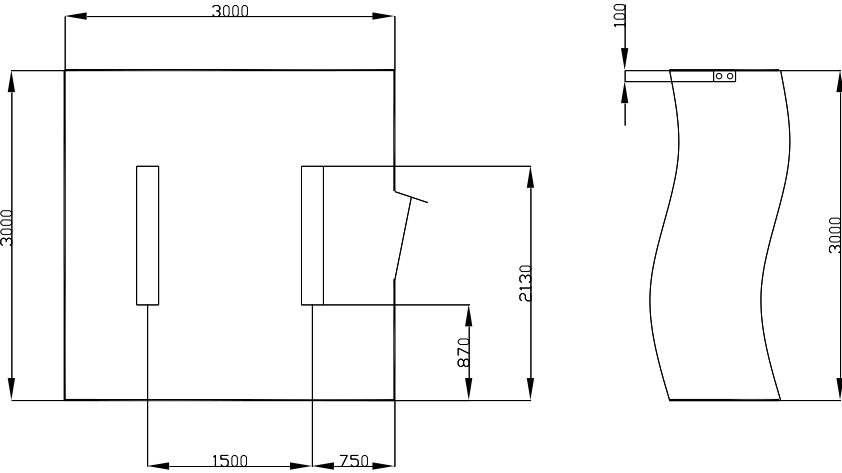
\includegraphics[width=\textwidth]{inc/light.png}
\caption{План размещения светильников в машинном зале}
\label{fig:light}
\end{figure}

Суммарная мощность светильников: $30\cdot4=160$ Вт. Суммарный световой поток: $1940\cdot4=7760$ лм.

Режим труда и отдыха должен зависеть от характера работы: при вводе данных, редактировании программ, чтении информации с экрана непрерывная продолжительность работы с монитором не должна превышать 4 часов. При 8 часовом рабочем дне, через каждый час работы необходимо проводить перерыв 5--10 минут, а каждые два часа перерыв в 15 мин.


\backmatter %% Здесь заканчивается нумерованная часть документа и начинаются ссылки и
            %% заключение

\chapter{Заключение}

В результате проделанной работы был проведен обзор системы моделирования GPSS и решены следующие задачи:

\begin{itemize}
\item Обоснован выбор подмножества блоков GPSS, реализуемых в работе.
\item Разработан и реализован алгоритм формирования моделей.
\item Реализованы алгоритмы имитационного моделирования сформированных моделей.
\item Разработаны аналитическая и имитационная модель типовой системы.
\item Реализована библиотека имитационного моделирования на языке Haskell.
\item Реализована демонстрационная программа, позволяющая оценить возможности разработанной библиотеки и оценить точность выбранных методов.
\item Проведено сравнение результатов аналитического и имитационного моделирования типовой системы, что подтвердило корректность реализации разработанной библиотеки.


\end{itemize}


% % Список литературы при помощи BibTeX
% Юзать так:
%
% pdflatex rpz
% bibtex rpz
% pdflatex rpz

\bibliographystyle{gost780u}
\bibliography{rpz}

%%% Local Variables: 
%%% mode: latex
%%% TeX-master: "rpz"
%%% End: 


\appendix   % Тут идут приложения
	

\end{document}

%%% Local Variables:
%%% mode: latex
%%% TeX-master: t
%%% End:
